% natbib options must be passed BEFORE the class, because cas-dc loads natbib itself
\PassOptionsToPackage{numbers,sort&compress}{natbib}

\documentclass[a4paper,fleqn]{cas-dc}

% --- Math ---
\usepackage{amsmath,amssymb}

% --- Graphics & figures ---
\usepackage{graphicx}
\usepackage{tikz}
\usepackage{pgfplots}
\pgfplotsset{compat=1.18}
\usetikzlibrary{positioning,arrows.meta,fit,shapes.geometric,calc,backgrounds,decorations.pathreplacing}

% --- Tables ---
\usepackage{array}
\usepackage{booktabs}
\usepackage{tabularx}

% --- Page layout / floats / landscape ---
\usepackage{rotating}
\usepackage{pdflscape}
\usepackage{placeins}

% --- Units ---
\usepackage{siunitx}

% --- Algorithms ---
\usepackage{algorithm}
\usepackage{algpseudocode}
\algrenewcommand\algorithmicrequire{\textbf{Input:}}
\algrenewcommand\algorithmicensure{\textbf{Output:}}

% --- Bibliography (options already passed above) ---
\usepackage{natbib}

% --- Springer (sn-jnl) commands used in the text but not defined by cas-dc ---
\providecommand{\botrule}{\bottomrule}
\providecommand{\backmatter}{}
\providecommand{\bmhead}[1]{\section*{#1}}

% --- Hyperref: cas-dc already loads it, so only set options here ---
\usepackage{hyperref}
\hypersetup{
    colorlinks = true,
    citecolor  = red,
    linkcolor  = blue,
    urlcolor   = magenta
}

\newcommand{\pgo}{\textsc{go}}
\newcommand{\pstop}{\textsc{stop}}
\newcommand{\pask}{\textsc{ask}}


\begin{document}
\let\WriteBookmarks\relax
\def\floatpagefraction{1}
\def\textpagefraction{.001}
\renewcommand{\topfraction}{0.9}\renewcommand{\dbltopfraction}{0.9}
\renewcommand{\floatpagefraction}{0.75}\renewcommand{\dblfloatpagefraction}{0.75}

\shorttitle{Coordinating questions to a shared operator with a calibrated QUBO}

\title[mode=title]{Coordinating Human Assistance in Multi-Robot Fleets: A QUBO Framework for Joint Go, Yield, and Ask Decisions}

\author[1]{Daniel Udekwe}
\ead{daudekwe@afit.edu.ng}

\author[1]{Qianwen Guo}
\ead{qguo@eng.famu.fsu.edu}
\cormark[1]




\affiliation[1]{organization={Department of Civil \& Environmental Engineering, FAMU-FSU College of Engineering},
                 city={Tallahassee},
                 postcode={32310},
                 state={Florida},
                 country={USA}}


\cortext[cor1]{Corresponding author}
\shortauthors{Udekwe (2026)}

\begin{abstract}
As delivery robots become increasingly deployed in shared environments, their ability to coordinate decisions and access limited human assistance is essential for safe and efficient operation. However, when multiple robots share a remote operator, independent go, yield, and ask decisions can generate competing requests and inefficiently allocate human attention. Existing decision-making approaches provide limited support for jointly optimizing these actions while accounting for pedestrian uncertainty, operator capacity, and response reliability. This study develops a joint decision-making framework for coordinating go, yield, and ask actions across delivery-robot fleets. The framework formulates the coordination problem as a quadratic unconstrained binary optimization (QUBO) model incorporating individual robot risks, action costs, and pairwise competition for operator attention. Its performance is evaluated using an exhaustive classical solver in closed-loop simulations, while a pre-specified quantum approximate optimization algorithm (QAOA) benchmark independently examines the optimization formulation. Joint optimization reduced decision delay relative to matched per-robot decision-making under perfect operator responses, with no collisions observed in these experiments, although a post-hoc analysis attributes most of this reduction to deferring every robot's decision to a common deadline rather than to joint optimization itself. Under imperfect operator responses, however, the joint solver produced more collisions, and collision non-inferiority was not established. QAOA outperformed uniform sampling across all benchmark instances, although its gains primarily reflected a preference for halt actions rather than effective coordination of assistance requests. Gazebo experiments further assessed consistency between offline predictions and simulated robot execution. These findings demonstrate the potential of joint optimization for coordinating human assistance across robot fleets while highlighting operator reliability and safety under uncertainty as critical considerations for practical deployment.


\end{abstract}

\begin{keywords}
Delivery robots \sep Human-robot interaction \sep Remote operation \sep Calibration \sep QUBO \sep Quantum approximate optimization algorithm
\end{keywords}

\maketitle


\section{Introduction}
\label{sec:intro}

Sidewalk delivery robots share space with pedestrians on university campuses and in city centres \citep{jennings2019sidewalk}. When a pedestrian stands near a robot's path, the robot cannot always tell whether the person is about to cross. Driving on risks a collision, and yielding to everyone wastes time. A third option is to ask: a remote operator who watches the robot's camera can say what the pedestrian is doing. Robots that ask humans for help are an old idea \citep{fong2003asker}, and recent work shows that asking only when the robot's own uncertainty is high saves human effort \citep{ren2023knowno}.

In earlier work we made this decision for a single robot \citep{udekwe2026askoract}. A predictor gives the probability that the pedestrian will cross, calibration makes that probability trustworthy, and at a decision deadline the robot goes, yields or asks according to where the calibrated probability falls. The rule is optimal when robots share nothing. A delivery fleet, however, usually shares one remote operator, who answers questions one at a time. If six robots ask at once, the last one waits for five answers, and a question that times out leaves the robot in a cautious fallback. Each robot's best action then depends on how many others ask, and per-robot thresholds are no longer optimal.

This paper studies that coupling. Its starting point is that the joint decision of all robots that reach their deadlines together is a quadratic binary optimization problem: the cost of each robot's action comes from its calibrated probability, and the operator's queue adds a cost for every pair of robots that ask. Problems of this form are exactly the class addressed by the quantum approximate optimization algorithm (QAOA) \citep{farhi2014qaoa}, and they arrive with coefficients from a real perception pipeline instead of the synthetic graphs common in QAOA benchmarks \citep{abbas2024challenges}. We therefore use the problem for two purposes: to measure what coordination buys a fleet, and to benchmark QAOA on perception-derived instances, in simulation and on IBM hardware.

We do not claim a quantum advantage. With at most eight robots in one decision epoch, exhaustive search over the $3^N$ joint actions takes milliseconds, and that exact solver is the joint policy in all closed-loop experiments. QAOA is the object of study in the benchmark, not a requirement of the fleet.

The contributions are as follows.
\begin{enumerate}
\item A QUBO formulation of the fleet's go, yield and ask decisions, with a pairwise queue term that prices the shared operator's service time. It needs exactly $2N$ binary variables, contains the single-robot rule as the uncoupled case, and also accounts for imperfect operator answers.
\item A closed-loop evaluation, following an analysis plan frozen before any final run, of what the joint solver buys over per-robot rules that ask equally often. This includes a pre-specified hypothesis that was not supported, and an explanation of why.
\item A pre-specified QAOA benchmark on these instances, in noiseless simulation (8 to 16 qubits) and on the 156-qubit \textit{ibm\_kingston} processor (8 and 12 qubits), with an exact classical reference for every instance.
\item A validation of the closed-loop simulator against Gazebo with several TurtleBot3 robots, using agreement criteria fixed in advance.
\item Post-hoc analyses, clearly separated from the confirmatory ones, of how much the safety results can support, of operator errors in both directions with answers drawn per question, of a risk-capped formulation, of offline--Gazebo agreement in near-collision encounters, of the sensitivity to answer accuracy and to the collision cost, and of QAOA against stronger classical and restricted-uniform baselines.
\end{enumerate}

Section~\ref{sec:related} reviews related work. Section~\ref{sec:method} describes the setting, the formulation, the solvers, the simulator and the analysis plan. Section~\ref{sec:results} reports the results, Section~\ref{sec:discussion} discusses them and their limitations, and Section~\ref{sec:conclusion} concludes.


\section{Related work}
\label{sec:related}

\paragraph{Multi-robot task allocation.}
Multi-robot task allocation assigns robots to tasks so as to optimize a team objective, and its taxonomies distinguish single- and multi-task robots, instantaneous and time-extended assignment, and independent and interdependent utilities \citep{gerkey2004taxonomy,korsah2013taxonomy}. Our problem inverts the usual roles: the scarce resource is not a robot but one human, and the ``tasks'' are the robots' own questions. It is an instantaneous assignment with interdependent utilities, because each question's value depends on how many others are asked in the same window.

\paragraph{Human attention allocation and operator scheduling.}
How many robots one person can supervise has been measured as fan-out, the ratio of a robot's autonomous time to the attention it needs \citep{olsen2004fanout}, and human-factors reviews document how operator workload, queueing and switching costs limit multi-robot supervision \citep{chen2014teaming}. Algorithmic work allocates operators to robots over time: \citet{dahiya2021operator} model it as a restless bandit, and \citet{swamy2020scaled} learn which robot an operator should control at each moment from the operator's own past choices. These methods schedule attention over long horizons, typically minutes to hours of fleet operation. We study a different, short-horizon decision: in a window of about one second, several robots reach a safety-relevant deadline together, and the question is which of them should ask at all, given that the operator answers one question at a time and that every robot that does not ask must go or yield immediately.

\paragraph{Robots that ask humans, and shared autonomy.}
Collaborative control treats the human as a resource that the robot may query when its own perception is unreliable \citep{fong2003asker}. More recent planners ask for help only when a calibrated uncertainty measure says the robot's choice is ambiguous, with statistical guarantees on how often they ask \citep{ren2023knowno}. Shared autonomy blends human input with the robot's own policy under uncertainty about the human's goal \citep{javdani2018shared}. In these works the human and the robot are paired; the coupling between robots that compete for one human, which is the subject of this paper, does not arise.

\paragraph{Pedestrian intent, calibration and decisions.}
Predicting whether a pedestrian will cross is a well-studied perception task \citep{rasouli2019pie}, and social navigation more broadly is surveyed by \citet{mavrogiannis2023core}. Modern neural predictors are often overconfident \citep{guo2017calibration}, and post-hoc methods such as isotonic regression \citep{zadrozny2002isotonic} restore calibration on average. Decision-focused learning argues that a predictor should be judged by the decisions it drives rather than by its average error \citep{elmachtoub2022spo}. In the single-robot setting we found that calibration measured over all samples can look good while the probabilities at the decision deadline remain poorly calibrated, and proposed decision-aware calibration fitted only on that window \citep{udekwe2026askoract}. Here we ask whether calibration still matters when the decision is made by an optimizer over several robots.

\paragraph{QUBO formulations and QAOA.}
Many combinatorial problems can be written as QUBO or Ising models \citep{lucas2014ising,glover2019qubo}. QAOA alternates a cost and a mixing Hamiltonian for $p$ layers and tunes the $2p$ angles classically \citep{farhi2014qaoa}. Parameter transfer between depths (the INTERP heuristic) makes optimization at larger $p$ tractable \citep{zhou2020qaoa}. Warm starts from a classical solution \citep{egger2021warm} and the conditional value at risk (CVaR) objective \citep{barkoutsos2020cvar} often improve results on constrained problems. Inequality constraints usually need slack qubits; unbalanced penalization avoids them at the risk of shifting the minimum \citep{montanez2024unbalanced}. Hardware studies show that QAOA's performance on current processors is limited by noise and by the routing overhead of problems that do not match the device's connectivity \citep{harrigan2021qaoa}. A recent review stresses that claims of quantum advantage in optimization need careful classical baselines \citep{abbas2024challenges}, and noisy intermediate-scale devices are not expected to beat classical solvers on small problems \citep{preskill2018nisq}.

\paragraph{Risk-sensitive and safety-constrained decisions.}
Minimizing expected cost trades rare severe outcomes against frequent small ones at a fixed exchange rate. Chance-constrained planning instead bounds the probability of failure directly \citep{blackmore2011chance}, and \citet{majumdar2020risk} argue that the choice of risk measure should itself be justified. Our main formulation minimizes expected cost, as the single-robot rule did; Section~\ref{sec:res-posthoc} adds a post-hoc comparison with a per-robot chance constraint.

\paragraph{Quantum optimization for multi-robot coordination.}
Quantum annealing has been used to route automated guided vehicles without collision \citep{ohzeki2019agv}, multi-robot path planning has been cast as a QUBO with problem-size reduction for current hardware \citep{gonzalez2026qubopath}, and \citet{petschnigg2019quantum} survey quantum computation for robotics. These studies coordinate robots' motion with synthetic or geometric costs. To our knowledge, none builds the QUBO coefficients from a calibrated perception model, couples robots through a shared human, or measures in closed loop how the resulting decisions affect safety and delay.

\section{Methodology}
\label{sec:method}

\begin{figure*}
\centering
\resizebox{\textwidth}{!}{%
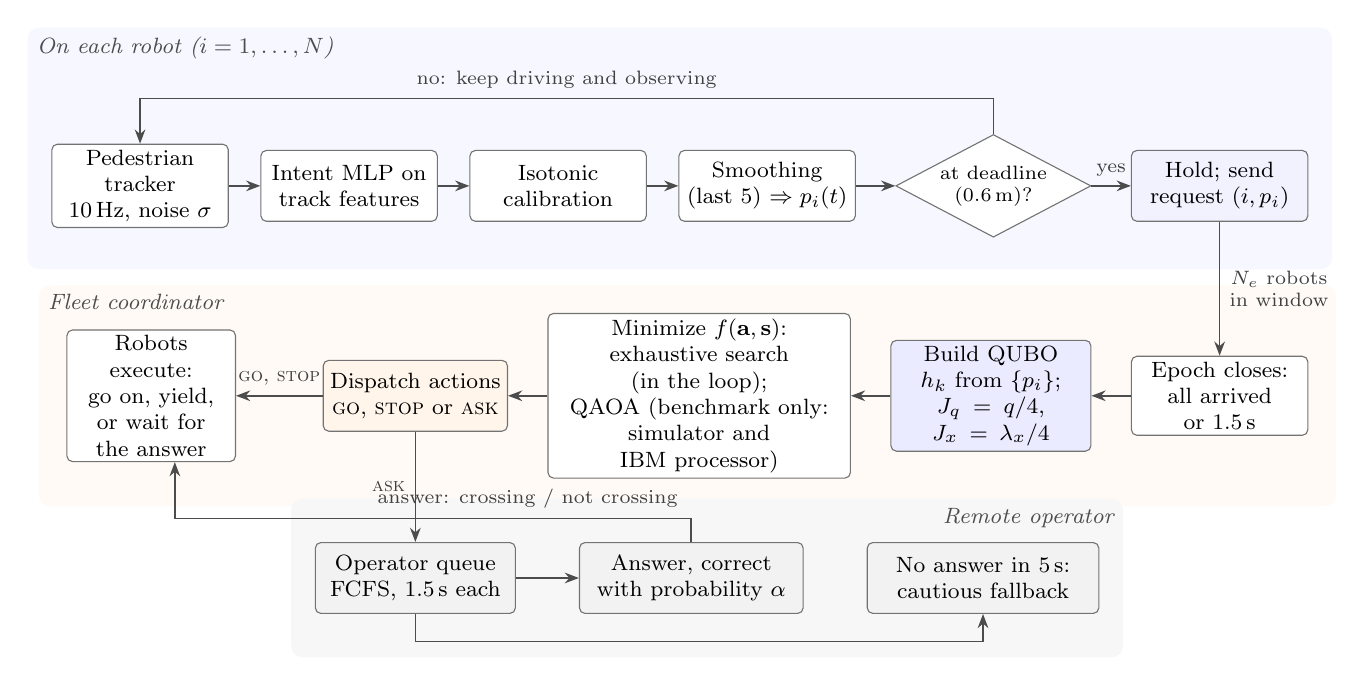
\begin{tikzpicture}[font=\footnotesize,
  box/.style={draw=black!55, rounded corners=2pt, align=center, fill=white, minimum height=9mm, text width=21mm, inner sep=2pt},
  dec/.style={draw=black!55, diamond, aspect=1.9, align=center, fill=white, inner sep=0.5pt, text width=14mm, font=\scriptsize},
  arr/.style={-{Stealth[length=1.8mm]}, draw=black!70, semithick},
  lbl/.style={font=\scriptsize, text=black!75, align=center},
  lane/.style={draw=none, rounded corners=4pt},
  ttl/.style={font=\footnotesize\itshape, text=black!70, anchor=north west}]
% robot lane
\node[box] (trk) at (0,0) {Pedestrian tracker\\\SI{10}{Hz}, noise $\sigma$};
\node[box, right=4mm of trk] (pred) {Intent MLP on\\track features};
\node[box, right=4mm of pred] (cal) {Isotonic\\calibration};
\node[box, right=4mm of cal] (sm) {Smoothing\\(last 5) $\Rightarrow p_i(t)$};
\node[dec, right=5mm of sm] (dl) {at deadline\\(\SI{0.6}{m})?};
\node[box, right=5mm of dl, text width=21mm, fill=blue!5] (hold) {Hold; send\\request $(i, p_i)$};
\draw[arr] (trk) -- (pred); \draw[arr] (pred) -- (cal); \draw[arr] (cal) -- (sm); \draw[arr] (sm) -- (dl);
\draw[arr] (dl) -- node[lbl, above] {yes} (hold);
\draw[arr] (dl.north) -- ++(0,0.45) coordinate (lt) -| node[lbl, pos=0.25, above] {no: keep driving and observing} (trk.north);
% coordinator lane
\node[box, below=17mm of hold, text width=21mm] (ep) {Epoch closes:\\all arrived or \SI{1.5}{s}};
\node[box, left=5mm of ep, fill=blue!8, text width=24mm] (qb) {Build QUBO\\$h_k$ from $\{p_i\}$;\\$J_q = q/4$, $J_x = \lambda_x/4$};
\node[box, left=5mm of qb, text width=37mm] (sv) {Minimize $f(\mathbf a,\mathbf s)$:\\exhaustive search (in the loop);\\QAOA (benchmark only:\\simulator and IBM processor)};
\node[box, left=5mm of sv, text width=22mm, fill=orange!8] (act) {Dispatch actions\\\pgo, \pstop\ or \pask};
\draw[arr] (hold) -- node[lbl, right] {$N_e$ robots\\in window} (ep);
\draw[arr] (ep) -- (qb); \draw[arr] (qb) -- (sv); \draw[arr] (sv) -- (act);
% operator lane
\node[box, below=14mm of act, text width=24mm, fill=black!5] (q) {Operator queue\\FCFS, \SI{1.5}{s} each};
\node[box, right=8mm of q, text width=27mm, fill=black!5] (ans) {Answer, correct\\with probability $\alpha$};
\node[box, right=8mm of ans, text width=28mm, fill=black!5] (to) {No answer in \SI{5}{s}:\\cautious fallback};
\draw[arr] (act) -- node[lbl, left] {\pask} (q);
\draw[arr] (q) -- (ans);
\draw[arr] (q.south) -- ++(0,-0.35) -| (to.south);
% execution back on robot
\node[box, left=11mm of act, text width=20mm] (exe) {Robots execute:\\go on, yield,\\or wait for\\the answer};
\draw[arr] (act) -- node[lbl, above] {\pgo, \pstop} (exe);
\draw[arr] (ans.north) -- ++(0,0.3) -| ($(exe.south)+(0.3,0)$);
\node[lbl, anchor=south east] at ($(ans.north)+(-0.05,0.3)$) {answer: crossing / not crossing};
\coordinate (ltop) at ($(lt)+(0,0.5)$);
% lanes
\begin{scope}[on background layer]
\node[lane, fill=blue!3, fit=(trk)(hold)(dl)(ltop), inner ysep=4mm, inner xsep=3mm] (L1) {};
\node[lane, fill=orange!4, fit=(exe)(act)(sv)(qb)(ep), inner sep=3.5mm] (L2) {};
\node[lane, fill=black!3, fit=(q)(ans)(to), inner ysep=5.5mm, inner xsep=3mm] (L3) {};
\end{scope}
\node[ttl] at (L1.north west) {On each robot ($i = 1,\dots,N$)};
\node[ttl] at (L2.north west) {Fleet coordinator};
\node[ttl, anchor=north east] at (L3.north east) {Remote operator};
\end{tikzpicture}}
\caption{Decision pipeline. On each robot, the tracked pedestrian's features feed an intent predictor whose output is calibrated and smoothed into a crossing probability $p_i$; the robot keeps driving and observing until the pedestrian is \SI{0.6}{m} ahead, then holds and sends its probability to the fleet coordinator. When the decision epoch closes, the coordinator builds the QUBO from the probabilities of all waiting robots, minimizes it, and sends each robot its action. Robots that ask join the operator's first-come-first-served queue; answers are correct with probability $\alpha$, and a question not answered within \SI{5}{s} falls back to the cautious rule. In the closed loop the QUBO is minimized exactly; QAOA is benchmarked offline on the same QUBOs.}
\label{fig:pipeline}
\end{figure*}

\subsection{Setting}
\label{sec:setting}

We consider a fleet of $N$ delivery robots on a campus, each driving its own route, supervised by one remote operator (Fig.~\ref{fig:pipeline}). Each robot uses the single-robot Ask or Act pipeline \citep{udekwe2026askoract}: it tracks the pedestrian ahead at \SI{10}{Hz}, a small neural network predicts the probability that the pedestrian will cross the robot's line, and isotonic calibration maps the raw score to a probability. The smoothed probability $p_i$ is updated at every observation. When a pedestrian is engaged (within \SI{1.0}{m} along the robot's line), the robot keeps driving and observing until the pedestrian is \SI{0.6}{m} ahead, the decision deadline, at which point it must choose one of three actions: go on (\pgo), yield (\pstop), or \pask\ the operator and hold until the answer arrives.

\paragraph{Decision epochs.} Robots that reach their deadlines within \SI{1}{s} of each other are decided together. A robot that arrives holds at its deadline until every other robot in the window has arrived or \SI{1.5}{s} has passed, whichever comes first; the joint solver then assigns an action to every waiting robot. A robot with no other robot in its window is decided alone, which reduces the joint problem to the single-robot rule.

\paragraph{The operator.} The operator answers questions one at a time, first come first served, in \SI{1.5}{s} each, and each answer is correct with probability $\alpha$. A question not answered within \SI{5}{s} falls back to the Ask or Act cautious rule (yield while the pedestrian is near the line). This is the only coupling between robots in our experiments: robots drive in separate lanes and never meet physically.

\subsection{Cost model and the per-robot rule}
\label{sec:cost}

Each robot's action is scored in units of robot-seconds. A collision costs $C$; yielding to a pedestrian who was not going to cross costs $\tau_s$; asking costs the robot's waiting time $\tau_a$ plus the operator's time $\kappa$, and, if answers can be wrong, the expected cost of acting on a wrong answer (Table~\ref{tab:confusion}). The pre-registered model counts only the more dangerous error, a crossing pedestrian reported as not crossing: With crossing probability $p_i$, the expected cost of each action is
\begin{align}
L_i(\pgo) &= C\,p_i, \nonumber\\
L_i(\pstop) &= \tau_s\,(1-p_i), \label{eq:unary}\\
L_i(\pask) &= \tau_a + \kappa + C\,p_i\,(1-\alpha). \nonumber
\end{align}
We fix $C = 100$, $\tau_s = 10$ and $\tau_a = 1.5$: a collision costs ten unnecessary stops, and a question holds the robot for about one service time. The operator's cost per question is $\kappa = 1.5$, so an operator-second is valued like a robot-second. Minimizing Eq.~\eqref{eq:unary} for one robot gives a threshold rule. With $\alpha = 1$ the robot goes if $p_i < (\tau_a+\kappa)/C = 0.03$, stops if $p_i > 1 - (\tau_a+\kappa)/\tau_s = 0.7$, and asks in between. With $\alpha<1$ the band becomes
\begin{equation}
\frac{\tau_a+\kappa}{\alpha\,C} < p_i < \frac{\tau_s - \tau_a - \kappa}{\tau_s + C(1-\alpha)},
\label{eq:band}
\end{equation}
and when the band is empty the robot goes below $p_i = \tau_s/(C+\tau_s)$ and stops above it. Sweeping $\kappa$ moves the band and with it how often a robot asks; we call these rules \emph{per-robot rules}. The original Ask or Act rule, with a fixed band $[0.2,\,0.8]$, is a further reference. Fig.~\ref{fig:costs} shows the three expected costs and the resulting bands for the primary parameters.

\paragraph{Operator errors.} The simulated operator errs symmetrically: whatever the pedestrian does, the answer is wrong with probability $1-\alpha$ (Table~\ref{tab:confusion}). A wrong ``not crossing'' answer about a crossing pedestrian sends the robot on and risks a collision; a wrong ``crossing'' answer about a pedestrian who was not going to cross makes the robot yield unnecessarily. The pre-registered ask cost in Eq.~\eqref{eq:unary} includes only the first outcome. The expected cost of asking under the full confusion model is
\begin{equation}
L_i^{\text{sym}}(\pask) = \tau_a + \kappa + (1-\alpha)\big[C\,p_i + \tau_s(1-p_i)\big],
\label{eq:asksym}
\end{equation}
which moves the asking band of Eq.~\eqref{eq:band} to
\begin{equation}
\frac{\tau_a+\kappa+(1-\alpha)\tau_s}{\alpha C+(1-\alpha)\tau_s} < p_i < \frac{\alpha\tau_s-\tau_a-\kappa}{\alpha\tau_s+(1-\alpha)C}
\label{eq:bandsym}
\end{equation}
($0.044 < p_i < 0.316$ at $\alpha = 0.9$, against $0.033 < p_i < 0.35$). With $\alpha = 1$ the two models coincide. All pre-registered results use Eq.~\eqref{eq:unary}; Section~\ref{sec:res-posthoc} repeats the imperfect-answer comparison with Eq.~\eqref{eq:asksym}.

\begin{table}
\centering
\caption{Operator confusion model and the outcome of each answer for a robot that asks. Each answer is correct with probability $\alpha$, independently of the pedestrian's intent.}
\label{tab:confusion}
\begin{tabular*}{\columnwidth}{@{\extracolsep{\fill}}lll}
\toprule
 Pedestrian & Answer ``crossing'' & Answer ``not crossing'' \\
\midrule
Crosses & $\alpha$: robot yields & $1-\alpha$: robot goes; \\
 & (no further cost) & risk, cost $C$ \\
Does not & $1-\alpha$: robot yields & $\alpha$: robot goes \\
cross & needlessly, cost $\tau_s$ & (no further cost) \\
\bottomrule
\end{tabular*}
\end{table}

\begin{figure*}
\centering
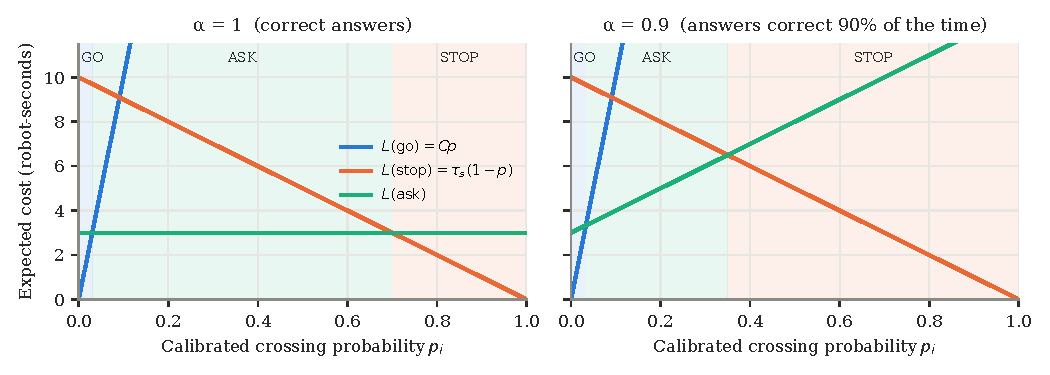
\includegraphics[width=\textwidth]{figures/costs.pdf}
\caption{Expected cost of each action for one robot as a function of its calibrated crossing probability (Eq.~\ref{eq:unary}; $C = 100$, $\tau_s = 10$, $\tau_a = \kappa = 1.5$). Shading marks the cheapest action. With perfect answers the robot asks for $0.03 < p_i < 0.7$; when answers are wrong 10\% of the time, asking carries part of the collision risk and the band shrinks to $0.033 < p_i < 0.35$.}
\label{fig:costs}
\end{figure*}

\subsection{The joint problem as a QUBO}
\label{sec:qubo}

Each robot $i$ in an epoch gets two binary variables: $a_i = 1$ if it asks and $s_i = 1$ if it stops; it goes when both are zero. If $k$ robots ask, the serial operator makes them wait $0, 1, \dots, k-1$ service times, a total of $k(k-1)/2$ service times, one for every pair of askers. With $q$ the cost of one service time of waiting ($q = 1.5$), the joint objective is
\begin{align}
f(\mathbf{a},\mathbf{s}) = \sum_{i=1}^{N} \Big[ &C\,p_i\,(1-a_i-s_i) + \tau_s(1-p_i)\,s_i \nonumber\\
 &+ \big(\tau_a+\kappa+C\,p_i(1-\alpha)\big)\,a_i \Big] \nonumber\\
 + q \sum_{i<j} a_i a_j &+ \lambda_x \sum_{i} a_i s_i .
\label{eq:qubo}
\end{align}
The last term forbids a robot from both asking and stopping; $\lambda_x$ is chosen large enough that no such state is ever optimal, which the test suite checks for every instance. The queue term is pairwise, so the problem is a QUBO in exactly $2N$ variables with no slack. With $q = 0$ it separates into the per-robot rule. The exclusion weight is set to $\lambda_x = 2\,(\Delta + q(N-1) + 1)$, where $\Delta$ is the spread of the unary costs, so that changing any one variable can never make a state with $a_i = s_i = 1$ cheaper than its feasible neighbours.

\paragraph{Ising form.} Writing $f = c_0 + \sum_k c_k x_k + \sum_{k<l} Q_{kl}\, x_k x_l$ over the $2N$ variables $x = (a_1,\dots,a_N,s_1,\dots,s_N)$ and substituting $x_k = (1 - Z_k)/2$ gives the cost Hamiltonian
% \begin{equation}
% H_C = c_0' + \sum_{k} h_k Z_k + \sum_{k<l} J_{kl}\, Z_k Z_l, \quad
% h_k = -\frac{c_k}{2} - \frac{1}{4}\sum_{l \ne k} Q_{kl}, \quad J_{kl} = \frac{Q_{kl}}{4}.
% \label{eq:ising}
% \end{equation}

\begin{equation}
\begin{aligned}
H_C &= c_0' + \sum_{k} h_k Z_k + \sum_{k<l} J_{kl}\, Z_k Z_l, \\
h_k &= -\frac{c_k}{2} - \frac{1}{4}\sum_{l \ne k} Q_{kl}, \\
J_{kl} &= \frac{Q_{kl}}{4}.
\end{aligned}
\label{eq:ising}
\end{equation}

For Eq.~\eqref{eq:qubo} the linear coefficients are $c_{a_i} = \tau_a + \kappa + C p_i(1-\alpha) - C p_i$ and $c_{s_i} = \tau_s(1-p_i) - C p_i$, so the calibrated probabilities enter only through the local fields $h_k$. The couplings do not depend on the probabilities: $J_q = q/4$ between every pair of ask qubits and $J_x = \lambda_x/4$ between each robot's ask and stop qubits. The interaction graph (Fig.~\ref{fig:circuit}b) is therefore a complete graph on the $N$ ask qubits with one pendant stop qubit per robot, $N(N+1)/2$ couplings in all (10, 21 and 36 at $N = 4$, 6 and 8).

\begin{figure*}
\centering
\begin{minipage}[b]{0.66\textwidth}\centering
\resizebox{\linewidth}{!}{%
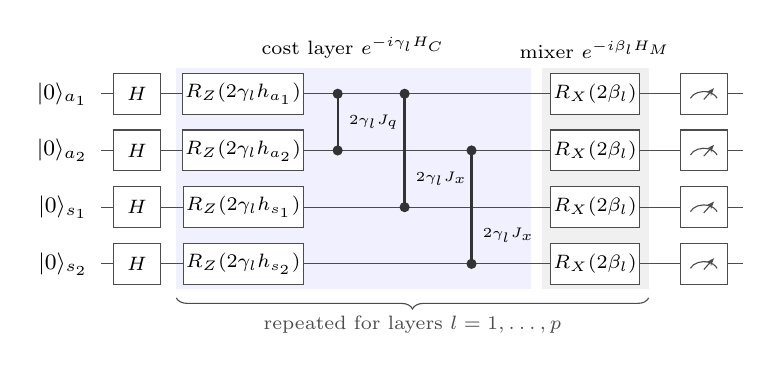
\begin{tikzpicture}[x=1cm,y=0.72cm,
  g/.style={draw=black!70, fill=white, minimum height=5.2mm, minimum width=8mm, inner sep=1pt, font=\scriptsize},
  dot/.style={circle, fill=black!80, inner sep=1.3pt}]
\foreach \y/\l in {0/{a_1},1/{a_2},2/{s_1},3/{s_2}} {
  \node[anchor=east, font=\footnotesize] at (-0.05,-\y) {$|0\rangle_{\l}$};
  \draw[black!70] (0,-\y) -- (8.15,-\y);
  \node[g, minimum width=6mm] at (0.45,-\y) {$H$};
}
\begin{scope}[on background layer]
\fill[blue!6] (0.95,0.45) rectangle (5.45,-3.45);
\fill[black!6] (5.6,0.45) rectangle (6.95,-3.45);
\end{scope}
\foreach \y/\l in {0/{a_1},1/{a_2},2/{s_1},3/{s_2}} \node[g, minimum width=15mm] at (1.8,-\y) {$R_Z(2\gamma_l h_{\l})$};
\draw[black!80, thick] (3.0,0) -- (3.0,-1); \node[dot] at (3.0,0) {}; \node[dot] at (3.0,-1) {};
\node[font=\tiny, anchor=west] at (3.02,-0.5) {$2\gamma_l J_{q}$};
\draw[black!80, thick] (3.85,0) -- (3.85,-2); \node[dot] at (3.85,0) {}; \node[dot] at (3.85,-2) {};
\node[font=\tiny, anchor=west] at (3.87,-1.5) {$2\gamma_l J_{x}$};
\draw[black!80, thick] (4.7,-1) -- (4.7,-3); \node[dot] at (4.7,-1) {}; \node[dot] at (4.7,-3) {};
\node[font=\tiny, anchor=west] at (4.72,-2.5) {$2\gamma_l J_{x}$};
\foreach \y in {0,1,2,3} \node[g, minimum width=11mm] at (6.27,-\y) {$R_X(2\beta_l)$};
\foreach \y in {0,1,2,3} {\node[g, minimum width=6mm] (m\y) at (7.65,-\y) {};
  \draw[black!70] ($(m\y.center)+(-0.17,-0.08)$) arc (160:20:0.18);
  \draw[black!70,-{Stealth[length=1mm]}] ($(m\y.center)+(0,-0.1)$) -- ++(0.13,0.2);}
\node[font=\scriptsize, anchor=south] at (3.2,0.45) {cost layer $e^{-i\gamma_l H_C}$};
\node[font=\scriptsize, anchor=south] at (6.27,0.45) {mixer $e^{-i\beta_l H_M}$};
\draw[decorate, decoration={brace, mirror, amplitude=4pt}, black!70] (0.95,-3.6) -- (6.95,-3.6)
  node[midway, below=3pt, font=\scriptsize] {repeated for layers $l = 1,\dots,p$};
\end{tikzpicture}}

\small (a)
\end{minipage}\hfill
\begin{minipage}[b]{0.3\textwidth}\centering
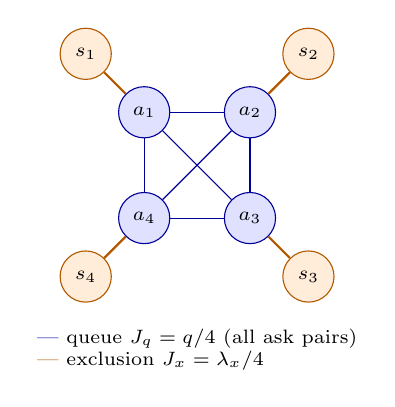
\begin{tikzpicture}[
  aq/.style={circle, draw=blue!60!black, fill=blue!12, minimum size=6.5mm, inner sep=0pt, font=\scriptsize},
  sq/.style={circle, draw=orange!70!black, fill=orange!15, minimum size=6.5mm, inner sep=0pt, font=\scriptsize}]
\foreach \i/\ang in {1/135,2/45,3/-45,4/-135} {
  \node[aq] (a\i) at (\ang:0.95) {$a_{\i}$};
  \node[sq] (s\i) at (\ang:2.0) {$s_{\i}$};
  \draw[orange!70!black, thick] (a\i) -- (s\i);
}
\foreach \i/\j in {1/2,1/3,1/4,2/3,2/4,3/4} \draw[blue!60!black] (a\i) -- (a\j);
\node[font=\scriptsize, align=left, anchor=north] at (0,-1.95) {\textcolor{blue!60!black}{---} queue $J_q = q/4$ (all ask pairs)\\ \textcolor{orange!70!black}{---} exclusion $J_x = \lambda_x/4$};
\end{tikzpicture}

\small (b)
\end{minipage}
\caption{(a) The QAOA circuit for a two-robot epoch (four qubits). After a Hadamard layer, each of $p$ layers applies the cost unitary, single-qubit $Z$ rotations carrying the probability-dependent fields $h_k$ and two-qubit $ZZ$ rotations for the queue ($J_q$) and exclusion ($J_x$) couplings, followed by $X$ rotations for the mixer; all qubits are then measured. (b) Interaction graph for $N = 4$: every pair of ask qubits is coupled by the operator queue, and each ask qubit is coupled to its robot's stop qubit.}
\label{fig:circuit}
\end{figure*}

\paragraph{Budget ablation.} As an ablation, the queue term is replaced by a hard cap of $B = \lceil N/3\rceil$ questions per epoch, $\sum_i a_i \le B$. For QAOA this needs either $K = \lceil\log_2(B+1)\rceil$ slack qubits $z_k$ with the penalty $\lambda_b(\sum_i a_i + \sum_k c_k z_k - B)^2$, or the unbalanced penalty $-\lambda_1\eta + \lambda_2\eta^2$ with $\eta = B - \sum_i a_i$ \citep{montanez2024unbalanced}, which needs no extra qubits but can move the minimum. Penalty weights were tuned on development instances only.

\subsection{Solvers}
\label{sec:solvers}

\paragraph{Exact.} Exhaustive search over the $3^N$ joint actions gives the optimum of every instance (59{,}049 action vectors at $N = 10$) and is the joint policy in all closed-loop experiments. OR-Tools CP-SAT \citep{ortools} and simulated annealing \citep{kirkpatrick1983sa} on the same QUBO were used during development as further references. The queue formulation is in fact classically easy, which we noticed only after the final runs. The queue cost depends only on the number $k$ of robots that ask, so for any $k$ the best choice is the $k$ robots with the largest saving $g_i = \min\{L_i(\pgo), L_i(\pstop)\} - L_i(\pask)$, and the optimum follows from sorting the savings and scanning $k = 0,\dots,N$ in $O(N \log N)$ time. This greedy allocation returned the optimum in every final instance and in 2{,}000 random ones. The coupling that makes the problem a QUBO is therefore benign; harder couplings, such as the corridor term or heterogeneous service times, would remove this shortcut.

\paragraph{QAOA circuit.} QAOA prepares the state
\begin{equation}
|\boldsymbol\gamma,\boldsymbol\beta\rangle = \prod_{l=1}^{p} e^{-i\beta_l H_M}\, e^{-i\gamma_l \tilde H_C}\, |+\rangle^{\otimes 2N},
\label{eq:qaoa}
\end{equation}
with the transverse-field mixer $H_M = \sum_k X_k$ \citep{farhi2014qaoa}. Before optimization the cost Hamiltonian is shifted and scaled by the mean $\mu$ and standard deviation $\sigma$ of its $2^{2N}$ eigenvalues, $\tilde H_C = (H_C - \mu)/\sigma$, so that angles have a comparable scale across instances. Because all terms of $\tilde H_C$ commute, the cost unitary is exact: $R_Z(2\gamma_l h_k/\sigma)$ on every qubit and $R_{ZZ}(2\gamma_l J_{kl}/\sigma)$ on every coupled pair; the mixer is $R_X(2\beta_l)$ on every qubit (Fig.~\ref{fig:circuit}a). One layer needs $2N$ $Z$ rotations, $N(N+1)/2$ two-qubit rotations and $2N$ $X$ rotations. On the heavy-hex connectivity of \textit{ibm\_kingston} each $R_{ZZ}$ becomes two CZ gates, and routing the complete ask-qubit graph adds SWAPs; after transpilation one layer used 27 CZ gates at $N = 4$ and 63 at $N = 6$, and two layers 58 and 149.

\paragraph{Parameter training.} The $2p$ angles minimize the expected normalized cost $F_p(\boldsymbol\gamma,\boldsymbol\beta) = \langle\boldsymbol\gamma,\boldsymbol\beta|\tilde H_C|\boldsymbol\gamma,\boldsymbol\beta\rangle$, computed exactly with a statevector simulator. We use COBYLA \citep{powell1994cobyla} (initial step 0.2, at most 400 evaluations) and grow the depth one layer at a time (Algorithm~\ref{alg:qaoa}). At depth 1 the optimizer starts from three random points with angles uniform in $[0, 0.8]$. At each further depth one start comes from the INTERP rule of \citet{zhou2020qaoa}, which interpolates the optimal depth-$p$ schedule onto $p+1$ layers,
\begin{equation}
\gamma_i^{(p+1)} = \frac{i-1}{p}\,\gamma_{i-1}^{(p)} + \frac{p-i+1}{p}\,\gamma_{i}^{(p)}, \quad i = 1,\dots,p+1,
\label{eq:interp}
\end{equation}
with $\gamma_0^{(p)} = \gamma_{p+1}^{(p)} = 0$ and the same rule for $\boldsymbol\beta$, and two come from random points; the best of the three is kept. Fig.~\ref{fig:landscape} shows the depth-1 landscape $F_1(\gamma,\beta)$ for one final instance. During development we also tested a warm start from each robot's own optimum \citep{egger2021warm} and a CVaR objective with level 0.1 \citep{barkoutsos2020cvar}. Neither was consistently better on the queue formulation, so the pre-specified benchmark uses the standard circuit. Circuits are built and transpiled with Qiskit \citep{javadi2024qiskit}, and the test suite checks that the statevector simulator reproduces Qiskit's statevector for the same circuits.

\begin{algorithm}
\caption{QAOA training with INTERP depth growth}
\label{alg:qaoa}
\begin{algorithmic}[1]
\Require normalized cost $\tilde H_C$; maximum depth $p_{\max}$; restarts $r = 3$
\Ensure angles $(\boldsymbol\gamma^{(p)},\boldsymbol\beta^{(p)})$ for $p = 1,\dots,p_{\max}$
\For{$p = 1,\dots,p_{\max}$}
  \State $\mathcal{S} \gets \emptyset$
  \If{$p > 1$} \State add $\mathrm{INTERP}(\boldsymbol\gamma^{(p-1)},\boldsymbol\beta^{(p-1)})$ to $\mathcal{S}$ \Comment{Eq.~\eqref{eq:interp}} \EndIf
  \State add random starts with angles in $[0, 0.8]$ until $|\mathcal{S}| = r$
  \State run COBYLA on $F_p$ from every start in $\mathcal{S}$
  \State $(\boldsymbol\gamma^{(p)},\boldsymbol\beta^{(p)}) \gets$ the run with the lowest $F_p$
\EndFor
\end{algorithmic}
\end{algorithm}

\begin{figure}
\centering
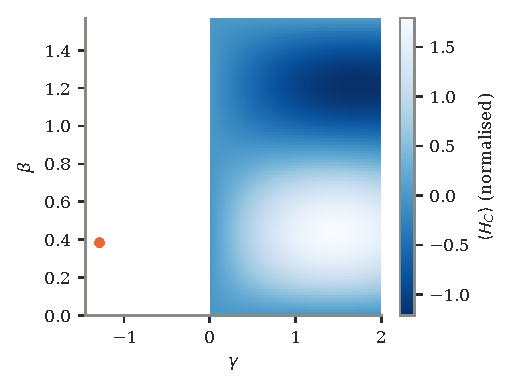
\includegraphics[width=\columnwidth]{figures/landscape.pdf}
\caption{Depth-1 landscape of the expected normalized cost $F_1(\gamma,\beta)$ for the first final instance with $N = 4$ (8 qubits). The marker is the optimum found by Algorithm~\ref{alg:qaoa}.}
\label{fig:landscape}
\end{figure}

\subsection{Calibrated probabilities}
\label{sec:probs}

The predictor and calibrators are those of Ask or Act \citep{udekwe2026askoract}: a multilayer perceptron on hand-crafted track features, recalibrated for each tracking condition by conventional isotonic regression (fitted on all samples) or by decision-aware isotonic regression (fitted only on samples near the decision deadline). We also report raw, uncalibrated scores. In the released single-robot code the smoothed probability stopped updating once the 40-observation history buffer was full, because predictions were cached on the buffer length. We corrected this before any result in this paper was produced; the probability now updates at every observation until the deadline.

\subsection{Closed-loop simulator}
\label{sec:sim}

The simulator runs the Ask or Act offline simulator for $N$ robots in lockstep at \SI{20}{Hz}, with a shared operator and decision epochs as above. Each robot drives at \SI{0.18}{m/s} along a \SI{5.8}{m} line and meets one scripted pedestrian from eight behaviour families, four crossing and four not crossing; hesitating and late-turning pedestrians, which appear in both groups, are deliberately ambiguous. A collision is a robot--pedestrian distance below \SI{0.4}{m}. Tracking noise has a standard deviation of \SI{0.03}{m} (nominal) or \SI{0.10}{m} (noisy). An epoch draws $N$ scenarios without replacement from the scenario pool and staggers the robots' arrivals at their deadlines uniformly over \SI{1}{s}. Every method sees the same scenarios, timing, tracker noise and operator answers in each epoch, so all comparisons are paired. Tracker noise and, in the pre-registered runs, the operator's answers are seeded per scenario, so a scenario that recurs in several epochs sees the same noise and the same answers. The two policy families also differ in when they decide. Per-robot rules run the Ask or Act threshold policy unchanged: a robot commits to going or stopping as soon as its smoothed probability leaves the asking band, and asks only at its deadline. Under the joint solver every robot observes until its deadline and then follows the joint assignment. For one robot the simulator reproduces the Ask or Act simulator exactly, which the test suite checks.

Algorithm~\ref{alg:epoch} summarizes one decision epoch for the joint solver.

\begin{algorithm}
\caption{One decision epoch with the joint solver}
\label{alg:epoch}
\begin{algorithmic}[1]
\Require robots $\mathcal{R}$ approaching their deadlines; window $w = \SI{1.5}{s}$; cost parameters $C,\tau_s,\tau_a,\kappa,q,\alpha$
\Ensure an action in $\{\pgo,\pstop,\pask\}$ for every robot in the epoch
\State $\mathcal{W} \gets \emptyset$; $t_0 \gets$ time the first robot reaches its deadline
\While{$t < t_0 + w$ \textbf{and} some robot in $\mathcal{R}\setminus\mathcal{W}$ is still approaching}
  \State add robots that reach their deadline to $\mathcal{W}$; each holds and records its calibrated $p_i$
\EndWhile
\State build $f$ in Eq.~\eqref{eq:qubo} from $\{p_i : i \in \mathcal{W}\}$
\State $(\mathbf{a}^\star,\mathbf{s}^\star) \gets \arg\min f$ \Comment{exhaustive over $3^{|\mathcal{W}|}$ actions}
\For{$i \in \mathcal{W}$}
  \State \textbf{if} $a_i^\star$ \textbf{then} send question to the operator queue; hold until answered or timeout
  \State \textbf{else if} $s_i^\star$ \textbf{then} yield \textbf{else} go
\EndFor
\end{algorithmic}
\end{algorithm}

\subsection{Pre-specified analysis plan}
\label{sec:plan}

All development used scenario seeds 4000--4099 and separate epoch seeds. The analysis plan, the final scripts and the code were then frozen, approved by both authors and tagged \texttt{v2-prereg} in the public repository before any run on the final seeds \citep{nosek2018prereg}. The final scenario pool (seeds 8000--8099, 800 scenarios per tracking condition) was built only after tagging.

\paragraph{Matched rules.} A joint solver that asks less would look better or worse for that reason alone. Each confirmatory comparison therefore uses a per-robot rule whose $\kappa^\star$ was set on development data so that it asks as often as the joint solver: $\kappa^\star = 5.95$ ($N = 6$) and 6.15 ($N = 8$) with $\alpha = 1$, and 6.04 and 6.20 with $\alpha = 0.9$ (using the $\alpha$-aware band of Eq.~\eqref{eq:band}). $\kappa^\star$ was not re-tuned on final data.

\paragraph{Hypotheses.} All closed-loop hypotheses use noisy tracking and decision-aware calibration, with 1{,}000 paired epochs.
\begin{itemize}
\item \textbf{H1} ($N = 6$, $\alpha = 1$): the joint solver gives lower mean delay per robot than the matched rule, with a collision rate on crossing robots at most 0.5 percentage points higher.
\item \textbf{H2} ($N = 8$, $\alpha = 1$): as H1.
\item \textbf{H3}: QAOA at depth 3 in noiseless simulation, on the queue formulation, places at least 10 times the uniform-random probability on the optimum, and its expected cost over feasible samples is below that of a uniformly random feasible state, in at least 80\% of 20 instances at each $N \in \{4,6,8\}$.
\item \textbf{H4} ($N = 6$, $\alpha = 0.9$): as H1, with the joint solver and the matched rule both accounting for $\alpha$.
\item \textbf{H5} ($N = 8$, $\alpha = 0.9$): as H4.
\end{itemize}
Delay is compared with a one-sided Wilcoxon signed-rank test on paired epoch means \citep{wilcoxon1945}, with Holm correction across the four closed-loop hypotheses (H1, H2, H4, H5) \citep{holm1979}. Collision non-inferiority requires the one-sided 95\% upper bound of the paired difference (joint minus rule), from an epoch-cluster bootstrap with 10{,}000 resamples \citep{efron1993bootstrap}, to lie below 0.5 percentage points. H3 is a descriptive criterion with Clopper--Pearson intervals \citep{clopper1934}. A further hypothesis comparing decision-aware with conventional calibration was moved to the exploratory list before freezing, because with the corrected probabilities no method collided with perfect answers on development data, leaving a collision test without events; H4 and H5 were added at the same time. The frozen plan numbers these hypotheses differently; the correspondence is given in the repository.

\paragraph{Exploratory analyses.} The plan lists, all to be reported: Pareto frontiers of the two policy families (33 methods, both tracking conditions, raw, conventional and decision-aware calibration); the fixed Ask or Act band; the budget ablation; the effect of calibration (exact McNemar test on paired crossing robots \citep{mcnemar1947}); and a joint solver that wrongly assumes perfect answers.

\paragraph{Hardware.} Forty circuits were pre-registered: 10 final instances at $N = 4$ and $N = 6$ (8 and 12 qubits), depths 1 and 2, parameters trained noiselessly, transpiled for \textit{ibm\_kingston} (IBM Heron r2, 156 qubits) at optimization level 3 keeping the best of 20 transpiler seeds, and 4{,}000 shots each, run in one batch with the sampler's default settings and no further error mitigation.

\paragraph{Gazebo validation.} Twenty final epochs with $N = 4$ TurtleBot3 robots in one Gazebo world \citep{koenig2004gazebo}, ROS~2 \citep{macenski2022ros2} and HuNavSim pedestrians \citep{perezhigueras2023hunavsim}, under both tracking conditions and with both the per-robot rule and the joint solver (320 robot runs), are compared with the offline simulator on identical inputs. The four criteria, set from a development validation, are: collision outcome agreement of at least 95\%; question-count agreement of at least 90\% for the per-robot rule; in at least 90\% of joint epochs, a Gazebo assignment that costs at most one question ($\tau_a + \kappa = 3$) more than the offline assignment under the offline probabilities; and a mean delay difference within \SI{\pm 0.5}{s} for every condition and method. The third criterion replaced raw action agreement before freezing, because in development the Gazebo robots reached their deadlines about \SI{0.14}{s} later than offline, and near-tied robots then swapped which of them asked.


\section{Results}
\label{sec:results}

\subsection{Confirmatory closed-loop results}
\label{sec:res-conf}

Table~\ref{tab:conf} reports the four closed-loop hypotheses. With perfect answers (H1 and H2), the joint solver saved about \SI{3}{s} per robot against the matched rule at both fleet sizes, and neither method collided in 3{,}321 ($N = 6$) and 4{,}538 ($N = 8$) encounters with a crossing pedestrian, so the non-inferiority criterion was met. Because these encounters came from only 400 distinct crossing scenarios, this is an encounter-level result (Section~\ref{sec:res-posthoc}, Table~\ref{tab:bounds}). The matched question rates differed by 7.7\% ($N = 6$) and 6.5\% ($N = 8$), within the pre-set 10\%. H1 and H2 are supported.

With answers correct 90\% of the time (H4 and H5), the joint solver was again about \SI{1.8}{s} faster, but it collided with 1.36\% ($N = 6$) and 1.04\% ($N = 8$) of crossing robots against none for the matched rule. The upper bounds of the difference, 1.68 and 1.28 percentage points, exceed the 0.5-point margin, so H4 and H5 are not supported. At $N = 8$ the two methods' question rates also differed by 15.8\%, more than the 10\% allowed; as pre-specified, this is reported as a deviation and $\kappa^\star$ was not re-tuned.

\begin{table*}
\centering
\caption{Confirmatory closed-loop results (noisy tracking, decision-aware calibration, 1{,}000 paired epochs each). Delay is mean delay per robot against free driving; collisions are per crossing robot. $p_{\text{Holm}}$: one-sided Wilcoxon on epoch means, Holm-corrected across the four rows. UB: one-sided 95\% bootstrap upper bound of the collision difference (joint $-$ rule); margin 0.5 percentage points (pp). Scenario-level bounds are given in Table~\ref{tab:bounds}.}
\label{tab:conf}
\begin{tabular*}{\textwidth}{@{\extracolsep{\fill}}llrrrrrrrrrl}
\toprule
 & & & \multicolumn{2}{c}{Questions/epoch} & \multicolumn{2}{c}{Delay (s)} & & \multicolumn{2}{c}{Collisions (\%)} & & \\
\cmidrule(lr){4-5}\cmidrule(lr){6-7}\cmidrule(lr){9-10}
Hyp. & $N$ & $\alpha$ & Joint & Rule & Joint & Rule & $p_{\text{Holm}}$ & Joint & Rule & UB (pp) & Supported \\
\midrule
H1 & 6 & 1.0 & 1.99 & 2.14 & 3.80 & 6.75 & $<10^{-160}$ & 0.00 & 0.00 & 0.00 & yes \\
H2 & 8 & 1.0 & 2.20 & 2.06 & 3.93 & 7.01 & $<10^{-160}$ & 0.00 & 0.00 & 0.00 & yes \\
H4 & 6 & 0.9 & 0.59 & 0.61 & 4.35 & 6.15 & $<10^{-160}$ & 1.36 & 0.00 & 1.68 & no \\
H5 & 8 & 0.9 & 0.75 & 0.63\rlap{$^{\dagger}$} & 4.34 & 6.11 & $<10^{-160}$ & 1.04 & 0.00 & 1.28 & no \\
\bottomrule
\multicolumn{12}{l}{\footnotesize $^{\dagger}$ Question rates differ by 15.8\%, more than the pre-set 10\%; reported as a deviation.}
\end{tabular*}
\end{table*}

\subsection{Operator load against delay}
\label{sec:res-pareto}

Fig.~\ref{fig:pareto} shows the two policy families as $\kappa$ is swept. At every question rate that both families reach, the joint solver is faster. The gap is largest at about two questions per epoch. A post-hoc decomposition (Section~\ref{sec:res-posthoc}, grey curve in Fig.~\ref{fig:pareto}) shows that almost all of this gap comes from when the decision is made rather than from deciding jointly. Robots facing a pedestrian who did not cross were stopped for 4.5 and \SI{4.9}{s} on average under the joint solver against 9.3 and \SI{10.2}{s} under the matched rule ($N = 6$ and 8).

The fixed Ask or Act band is the fastest method in the study (3.16 and \SI{3.26}{s}), also without collisions, but it asks three to four times as often as the joint solver (6.0 and 8.0 questions per epoch) and leaves 0.8 and 1.4 questions per epoch unanswered when the operator cannot keep up, against at most 0.003 for the joint solver. Its speed comes from operator time. Fig.~\ref{fig:epoch} shows how the two policies differ in one final epoch with six robots. The joint solver asked about two pedestrians whose probabilities were near the middle of the range (a late-turning pedestrian who crossed and one who did not), and let the operator answer both within \SI{3}{s}; the matched rule asked about three pedestrians, so its last robot waited for two earlier answers. Mean delay in this epoch was \SI{4.5}{s} under the joint solver and \SI{5.7}{s} under the rule. The joint solver is not better for every robot: robot R2, facing a hesitating pedestrian who did not cross ($p = 0.65$), was told to yield and waited \SI{8.4}{s}, whereas the rule asked and drove on after \SI{6.7}{s}.

\begin{figure*}
\centering
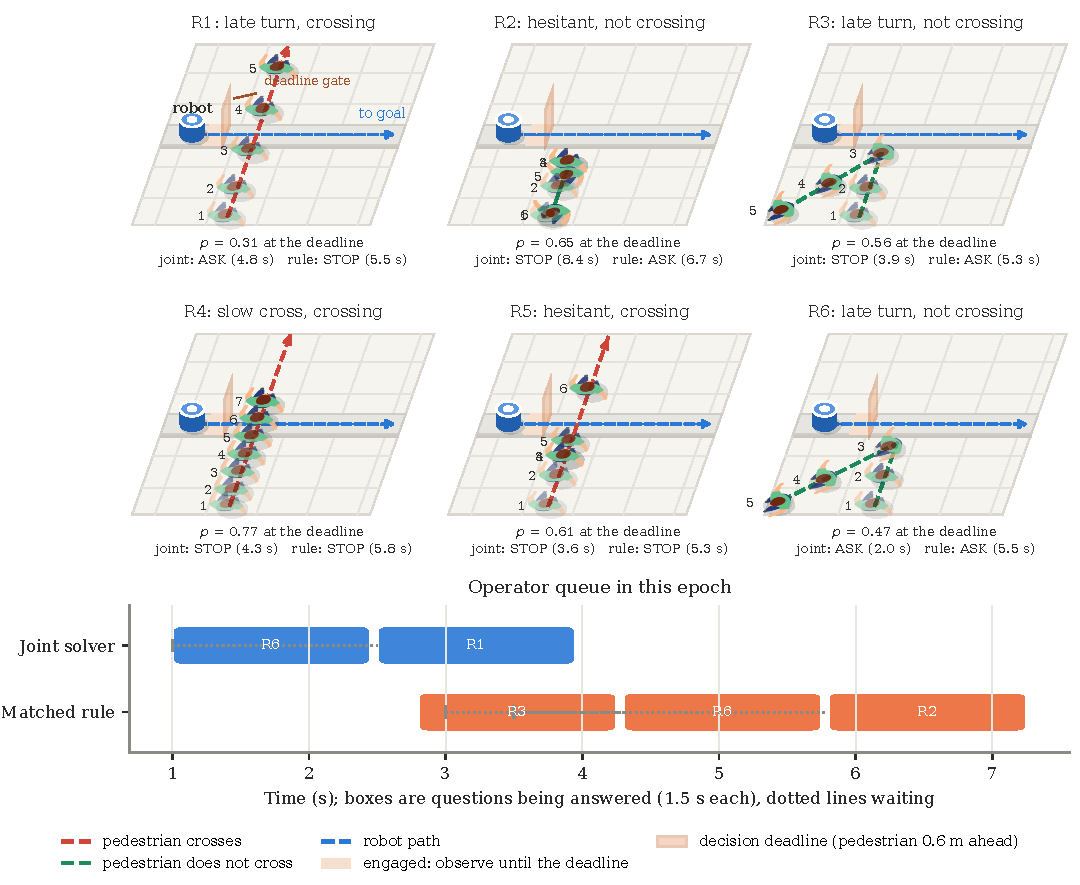
\includegraphics[width=\textwidth]{figures/epoch_3d.pdf}
\caption{One final decision epoch with six robots (noisy tracking, decision-aware calibration), drawn lane by lane in order of arrival at the decision deadline. Each lane shows the robot (a TurtleBot3) and its path, the stretch over which it observes the engaged pedestrian, its decision deadline (drawn as a gate where the pedestrian is \SI{0.6}{m} ahead), and the pedestrian's positions along its path, about \SI{1}{m} of walking apart (numbered in time order, fading for earlier times; pauses are labelled). Below each lane: the calibrated probability at the deadline and the action and delay under the joint solver and the matched per-robot rule. Bottom: the operator's queue under each policy. Robot and pedestrians are enlarged for visibility.}
\label{fig:epoch}
\end{figure*} Replacing the queue term by a hard budget of $\lceil N/3\rceil$ questions gave almost the same delay (3.81 and \SI{3.86}{s}) at 2.0 and 3.0 questions per epoch.

\begin{figure*}
\centering
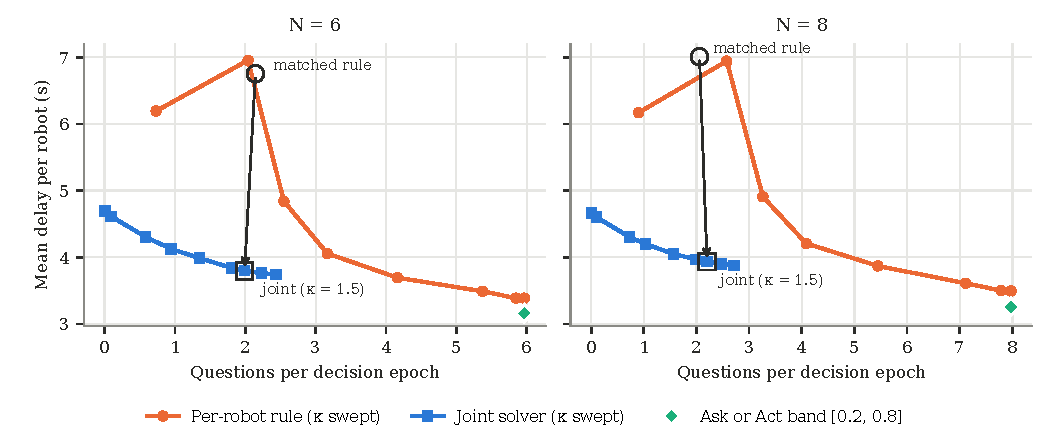
\includegraphics[width=\textwidth]{figures/pareto.pdf}
\caption{Questions per decision epoch against mean delay per robot, for the per-robot rule and the joint solver as the operator cost $\kappa$ varies (noisy tracking, decision-aware calibration, $\alpha = 1$, 1{,}000 epochs per point). The arrows join the matched pairs of H1 ($N = 6$) and H2 ($N = 8$). Grey (post hoc): the per-robot rule applied at the decision deadline, in the joint solver's execution mode (joint solver without the queue term, $\kappa$ swept). No method collided in these settings.}
\label{fig:pareto}
\end{figure*}

\subsection{Calibration and imperfect answers}
\label{sec:res-calib}

Table~\ref{tab:calib} shows collisions by calibration. With perfect answers the only collisions in the study occurred with raw, uncalibrated probabilities under noisy tracking: 0.30\% and 0.29\% of crossing robots for the joint solver, and similarly for every joint variant in the sweep. Both calibrations eliminated them. Between decision-aware and conventional calibration there was no difference with perfect answers (no collisions either way). With $\alpha = 0.9$ decision-aware calibration had the fewest collisions in every cell, but at $N = 6$ under noisy tracking the paired difference was not significant (12 against 20 discordant crossing robots, exact McNemar $p = 0.22$).

All joint variants that ask about pedestrians with moderate probabilities collided at $\alpha = 0.9$. With decision-aware calibration, $\alpha$-aware per-robot rules with $\kappa \ge 1.5$ never collided; with conventional or raw calibration the same rules collided with up to 1.4\% of crossing robots under noisy tracking, so calibration matters for the per-robot family too. A joint solver that wrongly assumes perfect answers had a collision rate similar to the $\alpha$-aware solver (1.42\% against 1.36\% at $N = 6$) while asking three times as often.

\begin{table}
\centering
\caption{Collisions per crossing robot (\%) for the joint solver, by calibration (exploratory; 1{,}000 epochs per cell; 3{,}321 crossing robots at $N = 6$, 4{,}538 at $N = 8$).}
\label{tab:calib}
\begin{tabular*}{\columnwidth}{@{\extracolsep{\fill}}lllrrr}
\toprule
$\alpha$ & Tracking & $N$ & Raw & Conv. & Dec.-aware \\
\midrule
1.0 & noisy & 6 & 0.30 & 0.00 & 0.00 \\
1.0 & noisy & 8 & 0.29 & 0.00 & 0.00 \\
1.0 & nominal & 6, 8 & 0.00 & 0.00 & 0.00 \\
0.9 & noisy & 6 & 1.78 & 1.60 & 1.36 \\
0.9 & noisy & 8 & 1.17 & 1.08 & 1.04 \\
0.9 & nominal & 6 & 0.54 & 0.15 & 0.00 \\
0.9 & nominal & 8 & 0.37 & 0.24 & 0.00 \\
\bottomrule
\end{tabular*}
\end{table}

\subsection{QAOA benchmark and hardware}
\label{sec:res-qaoa}

H3 was met at every size: all 20 instances passed at $N = 4$, 6 and 8 (share 1.0, Clopper--Pearson interval [0.83, 1.0]). Median lifts over uniform sampling were 15.8, 61.8 and 214.8 (Fig.~\ref{fig:qaoa}a). The feasible share of the QAOA state was 0.998, 0.997 and 0.986, and the expected cost of feasible samples was 26\%, 27\% and 37\% above the optimum, against 423--509\% for a uniformly random feasible state. During development, depth 3 was not enough at $N = 10$ (20 qubits), where the expected cost of feasible samples stayed about 185\% above the optimum.

\paragraph{What the trained circuits learn (post hoc).} Fig.~\ref{fig:qaoaparams} traces the trained circuits on the 60 final instances; this analysis was not pre-specified. The optimized schedules are similar across instances and sizes (panel a), and the INTERP growth converges in a few hundred evaluations at each depth (panel c). Panels (b) and (d) show what the lift measures. As depth grows, the state concentrates on the $2^N$ \emph{halt} states in which every robot either asks or stops (95--99.5\% of the probability at depth 3, against $2^{-N}$ under uniform sampling), and the lift approaches $2^N$ (16, 64 and 256). Inside that subspace the distribution is almost uniform: its total-variation distance from uniform is at most 0.03, and the optimum receives 0.96--0.99 times the probability of an average halt state. In every final instance the optimum is a halt state, so the circuits gain their lift by ruling out going (expensive at these probabilities) and the infeasible ask-and-stop states, not by choosing which robots should ask. The energy differences inside the halt subspace are small: the gap between the optimum and the next state is 0.3--0.75\% of the standard deviation of the spectrum, which is dominated by the go costs and the exclusion penalty, and one to three layers do not resolve it.

\begin{figure*}
\centering
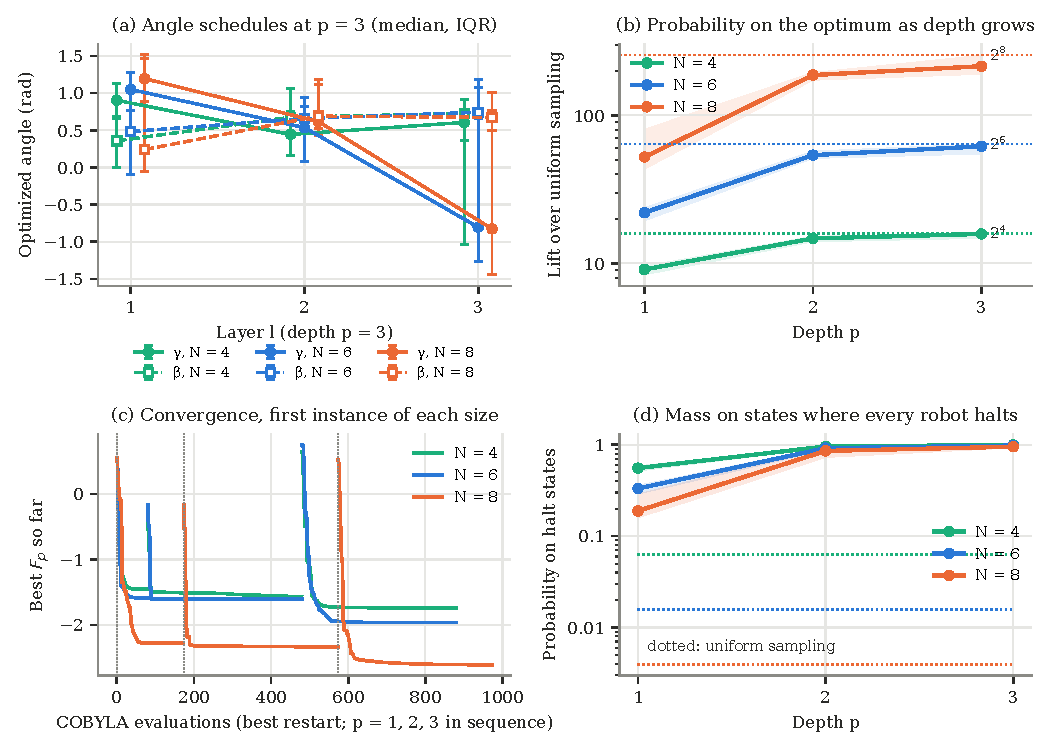
\includegraphics[width=\textwidth]{figures/qaoa_params.pdf}
\caption{QAOA training on the 60 final instances (noiseless). (a) Optimized angles of each layer at depth 3 (median and interquartile range over 20 instances per size). (b) Lift over uniform sampling as depth grows; dotted lines mark $2^N$. (c) Best expected normalized cost $F_p$ found by COBYLA during INTERP depth growth, for the first instance of each size. (d) Probability on the $2^N$ states in which every robot either asks or stops; dotted lines mark uniform sampling. Panels (b) and (d) are a post-hoc analysis.}
\label{fig:qaoaparams}
\end{figure*}

On \textit{ibm\_kingston} the optimum was sampled in all 40 circuits (Table~\ref{tab:hw}, Fig.~\ref{fig:qaoa}b). At $N = 4$ the hardware retained most of the noiseless lift (7.3 against 8.6 at depth 1, 11.6 against 15.3 at depth 2). At $N = 6$ the depth-1 circuit kept 20.0 of 26.4, but the depth-2 circuit, with 149 two-qubit gates after routing, reached only 22.5 against 55.4 noiselessly: noise removed most of the second layer's gain. The share of feasible samples stayed well above random at every size, but fell with depth on hardware.

\begin{figure*}
\centering
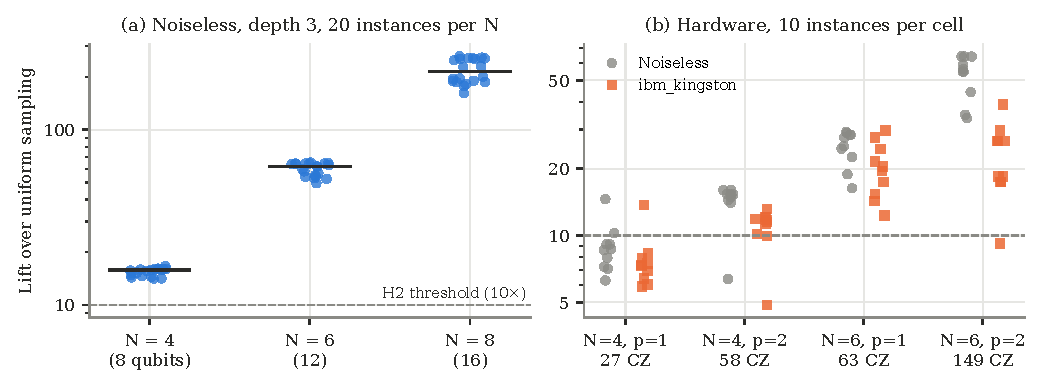
\includegraphics[width=\textwidth]{figures/qaoa.pdf}
\caption{QAOA on the queue formulation. (a) Lift over uniform sampling (probability on the optimum divided by its uniform probability) for 20 final instances per size, noiseless, depth 3; lines show medians, dashed line the pre-specified threshold. (b) The same quantity on \textit{ibm\_kingston} and in noiseless simulation for the 40 pre-registered circuits ($p$: QAOA depth; CZ: two-qubit gates after transpilation).}
\label{fig:qaoa}
\end{figure*}

\begin{table}
\centering
\caption{Hardware results on \textit{ibm\_kingston}, medians over 10 final instances, 4{,}000 shots each. Lift: probability on the optimum over its uniform probability. Feasible: share of samples with no robot both asking and stopping.}
\label{tab:hw}
\begin{tabular*}{\columnwidth}{@{\extracolsep{\fill}}rrrrrrrr}
\toprule
 & & & \multicolumn{2}{c}{Lift} & \multicolumn{3}{c}{Feasible} \\
\cmidrule(lr){4-5}\cmidrule(lr){6-8}
$N$ & $p$ & CZ & Sim. & HW & Sim. & HW & Rand. \\
\midrule
4 & 1 & 27 & 8.6 & 7.3 & 0.95 & 0.90 & 0.32 \\
4 & 2 & 58 & 15.3 & 11.6 & 0.99 & 0.88 & 0.32 \\
6 & 1 & 63 & 26.4 & 20.0 & 0.95 & 0.79 & 0.18 \\
6 & 2 & 149 & 55.4 & 22.5 & 0.98 & 0.69 & 0.18 \\
\bottomrule
\end{tabular*}
\end{table}

\subsection{Agreement with Gazebo}
\label{sec:res-gazebo}

All four pre-specified criteria were met on the final Gazebo epochs (Table~\ref{tab:gazebo}), with no runs excluded. Collision outcomes agreed in all 320 robot runs (no collisions on either side). In joint mode, 88\% of robots received the same action as offline. The disagreements were between near-tied robots: in all 40 joint epochs the Gazebo assignment cost at most 2.15 units more than the offline one under the offline probabilities, less than one question.

\begin{table}
\centering
\caption{Gazebo against the offline simulator on the 20 final epochs ($N = 4$; 80 robot runs per row).}
\label{tab:gazebo}
\begin{tabular*}{\columnwidth}{@{\extracolsep{\fill}}llrrrr}
\toprule
Tracking & Method & Coll. & Quest. & Action & $\Delta$delay (s) \\
\midrule
noisy & rule & 1.00 & 0.98 & 1.00 & 0.14 \\
noisy & joint & 1.00 & 0.89 & 0.88 & 0.20 \\
nominal & rule & 1.00 & 1.00 & 1.00 & 0.12 \\
nominal & joint & 1.00 & 0.89 & 0.89 & 0.10 \\
\bottomrule
\end{tabular*}
\end{table}

\subsection{Post-hoc analyses}
\label{sec:res-posthoc}

The analyses in this subsection were added after the final results had been obtained, in response to review. None was pre-specified, and they do not change which hypotheses were supported. They use the final scenario pool and the same final epochs as the confirmatory runs unless stated otherwise.

\paragraph{What zero collisions show.} The epochs reuse scenarios: at $N = 6$ the 3{,}321 encounters with a crossing pedestrian came from only 400 distinct crossing scenarios, each used about eight times with the same tracker noise. Table~\ref{tab:bounds} therefore gives two bounds. With no collision in 3{,}321 encounters, the one-sided 95\% Clopper--Pearson bound on the collision rate per encounter is 0.090\% (0.066\% at $N = 8$), well inside the 0.5-point margin. If the 400 scenarios are taken as the independent units, the bound is 0.75\%, outside the margin; about 600 distinct crossing scenarios without a collision would be needed to show non-inferiority at that level. The H1 and H2 safety result is thus an encounter-level statement about this scenario pool, not evidence that the joint solver is as safe as the rule on unseen scenarios. For H4 and H5 the collisions came from seven and eight scenarios; resampling scenarios rather than epochs raises the upper bound of the difference from 1.69 to 2.30 points ($N = 6$) and from 1.29 to 1.75 points ($N = 8$).

\begin{table*}
\centering
\caption{Collision uncertainty in the confirmatory runs (noisy tracking, decision-aware calibration, 1{,}000 epochs). Encounters: robots whose pedestrian crossed; scenarios: distinct crossing scenarios among them. UB: one-sided 95\% upper bound. Rate bounds are Clopper--Pearson, per encounter or, for the share of scenarios with a collision, per scenario. Difference bounds (joint $-$ rule, percentage points) use the bootstrap with epochs or scenarios resampled. The rule had no collisions in any row.}
\label{tab:bounds}
\begin{tabular*}{\textwidth}{@{\extracolsep{\fill}}lrrrrrrrrr}
\toprule
 & & & & & \multicolumn{2}{c}{Joint UB (\%)} & & \multicolumn{2}{c}{Difference UB (pp)} \\
\cmidrule(lr){6-7}\cmidrule(lr){9-10}
Hyp. & $N$ & $\alpha$ & Encounters & Scenarios & Encounter & Scenario & Joint coll. (scen.) & Epochs & Scenarios \\
\midrule
H1 & 6 & 1.0 & 3{,}321 & 400 & 0.090 & 0.75 & 0 (0) & 0.00 & 0.00 \\
H2 & 8 & 1.0 & 4{,}538 & 400 & 0.066 & 0.75 & 0 (0) & 0.00 & 0.00 \\
H4 & 6 & 0.9 & 3{,}321 & 400 & 1.73 & 3.26 & 45 (7) & 1.69 & 2.30 \\
H5 & 8 & 0.9 & 4{,}538 & 400 & 1.32 & 3.58 & 47 (8) & 1.29 & 1.75 \\
\bottomrule
\end{tabular*}
\end{table*}

\paragraph{Independent answers and the full confusion model.} We repeated the $\alpha = 0.9$ comparison with each answer drawn independently per question, first with the pre-registered cost model and the pre-registered $\kappa^\star$, and then with the symmetric ask cost of Eq.~\eqref{eq:asksym}, for which $\kappa^\star$ of the per-robot rule was matched again on development seeds (5.42 at $N = 6$, 5.54 at $N = 8$). Table~\ref{tab:posthoc} and Fig.~\ref{fig:safety} give the results. With independent answers and the pre-registered model, the joint solver collided with 12 crossing robots at each size (0.36\% and 0.26\%), spread over ten scenarios, against 45 and 47 with answers reused per scenario; the bound of the difference fell to 0.54 and 0.40 points, still above the margin at $N = 6$. With the symmetric model the joint solver asked less often, because a wrong ``crossing'' answer now costs an unnecessary stop, and collided with 7 and 9 crossing robots (0.21\% and 0.20\%). The bounds of the difference were 0.34--0.37 points at $N = 6$ and 0.31--0.35 points at $N = 8$, inside the margin whether epochs or scenarios are resampled, and the joint solver remained \SI{1.7}{s} faster per robot. Under this post-hoc design the joint solver would therefore meet the non-inferiority criterion, although the matched rule still had no collisions. Two caveats apply: the matching of question rates transferred less well from development than before (the rule asked 23\% more often than the joint solver at $N = 6$ and 12\% less often at $N = 8$), and with nominal tracking neither method collided in any variant.

\paragraph{Bounding collision risk directly.} A chance constraint on each robot, $P(\text{collision}_i \mid a_i) \le \varepsilon$, can be added without leaving the QUBO class: going carries risk $p_i$, asking $p_i(1-\alpha)$ and stopping none, so each constraint simply removes actions from a robot's choice set. Table~\ref{tab:posthoc} reports the symmetric joint solver with $\varepsilon \in \{0.005, 0.01, 0.02\}$. Under noisy tracking, $\varepsilon \le 0.01$ removed every collision, but also every question. The cap allows going only for $p_i \le \varepsilon$ and asking only for $p_i \le 10\varepsilon$, and with noisy tracking the calibrated probability at the deadline was at least 0.15 for every pedestrian in the final pool, so every robot stopped. This all-stop policy was nevertheless \SI{1.4}{s} faster than the matched rule (4.69 against \SI{6.13}{s} at $N = 6$); the reason is examined below. With $\varepsilon = 0.02$ the solver asked 16 and 20 questions in 1{,}000 epochs, and 3 and 1 of them ended in collisions. In this problem a tight risk cap turns the joint solver into a cautious go-or-stop rule, so the operator is used only when the cap is loose enough to tolerate the collision risk of a wrong answer. The expected-cost and risk-capped formulations mark two ends of a trade-off that the operator's accuracy decides.

\begin{table*}
\centering
\caption{Post-hoc imperfect-answer comparison (noisy tracking, decision-aware calibration, $\alpha = 0.9$, answers drawn independently per question, 1{,}000 epochs). Collisions are per crossing robot, with the number of distinct scenarios in parentheses; UB: one-sided 95\% bootstrap upper bound of the difference from the matched rule of the same cost model (pp), with epochs or scenarios resampled. Pre-registered and symmetric: ask cost of Eq.~\eqref{eq:unary} or Eq.~\eqref{eq:asksym}. Stopped: mean stopped time of robots whose pedestrian did not cross. $\varepsilon = 0.005$ gave the same results as $\varepsilon = 0.01$.}
\label{tab:posthoc}
\begin{tabular*}{\textwidth}{@{\extracolsep{\fill}}llrrrrrrr}
\toprule
 & & & & & & & \multicolumn{2}{c}{Difference UB (pp)} \\
\cmidrule(lr){8-9}
$N$ & Method & Quest./epoch & Delay (s) & Stopped (s) & Collisions & (\%) & Epochs & Scenarios \\
\midrule
6 & Joint, pre-registered & 0.59 & 4.35 & 5.76 & 12 (10) & 0.36 & 0.54 & 0.56 \\
  & Rule, pre-registered ($\kappa^\star = 6.04$) & 0.61 & 6.15 & 7.76 & 0 & 0.00 & -- & -- \\
  & Joint, symmetric & 0.39 & 4.44 & 5.96 & 7 (6) & 0.21 & 0.34 & 0.37 \\
  & Rule, symmetric ($\kappa^\star = 5.42$) & 0.49 & 6.13 & 7.71 & 0 & 0.00 & -- & -- \\
  & Joint, sym., $\varepsilon = 0.01$ & 0.00 & 4.69 & 6.52 & 0 & 0.00 & 0.00 & 0.00 \\
  & Joint, sym., $\varepsilon = 0.02$ & 0.02 & 4.69 & 6.52 & 3 (2) & 0.09 & 0.18 & 0.21 \\
\midrule
8 & Joint, pre-registered & 0.75 & 4.34 & 5.81 & 12 (10) & 0.26 & 0.40 & 0.42 \\
  & Rule, pre-registered ($\kappa^\star = 6.20$) & 0.63 & 6.11 & 7.75 & 0 & 0.00 & -- & -- \\
  & Joint, symmetric & 0.53 & 4.41 & 5.97 & 9 (7) & 0.20 & 0.31 & 0.35 \\
  & Rule, symmetric ($\kappa^\star = 5.54$) & 0.47 & 6.11 & 7.74 & 0 & 0.00 & -- & -- \\
  & Joint, sym., $\varepsilon = 0.01$ & 0.00 & 4.66 & 6.56 & 0 & 0.00 & 0.00 & 0.00 \\
  & Joint, sym., $\varepsilon = 0.02$ & 0.02 & 4.66 & 6.56 & 1 (1) & 0.02 & 0.07 & 0.07 \\
\bottomrule
\end{tabular*}
\end{table*}

\begin{figure*}
\centering
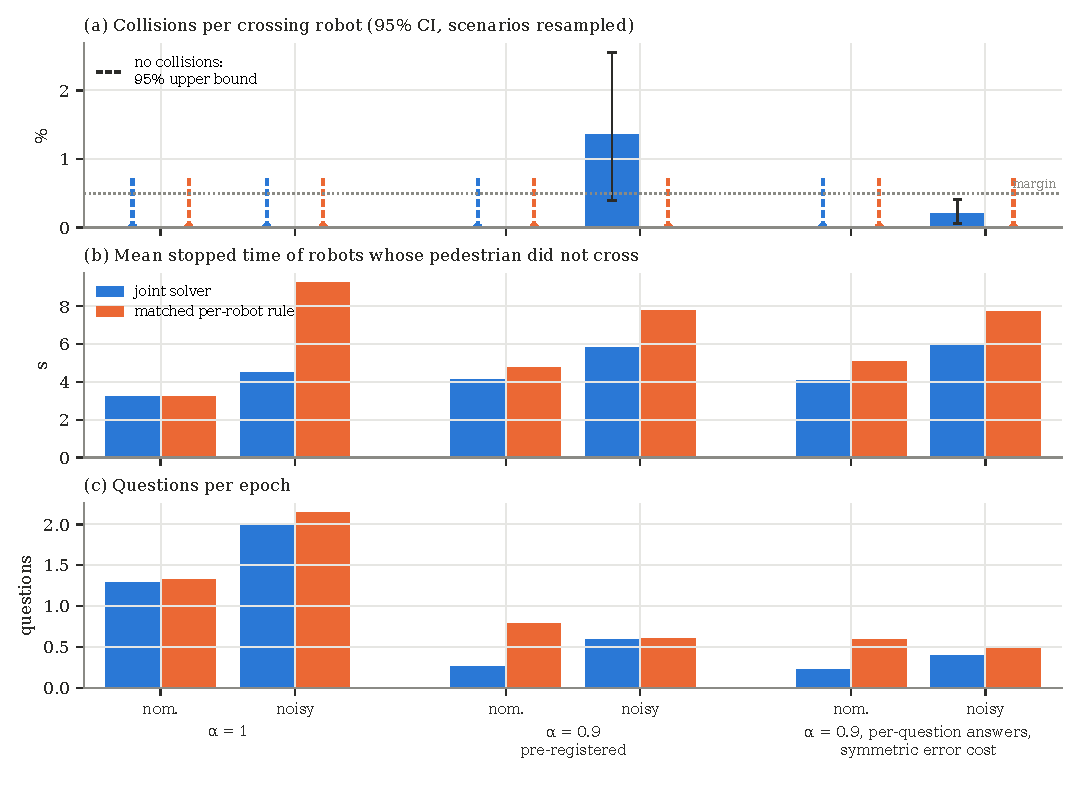
\includegraphics[width=\textwidth]{figures/safety.pdf}
\caption{Safety and its price at $N = 6$ (decision-aware calibration, 1{,}000 epochs per bar), for the joint solver and the matched per-robot rule under perfect answers, under the pre-registered imperfect-answer design (answers reused per scenario) and under the post-hoc design (answers drawn per question, symmetric error cost). (a) Collisions per crossing robot with 95\% intervals from resampling scenarios; where no collision occurred, the dashed line shows the one-sided 95\% Clopper--Pearson bound over the 400 distinct crossing scenarios, and the dotted line marks the 0.5-point margin. (b) Mean stopped time of robots whose pedestrian did not cross (unnecessary stopping). (c) Questions per epoch.}
\label{fig:safety}
\end{figure*}

\paragraph{Sensitivity to answer accuracy and collision cost.} Fig.~\ref{fig:sensitivity} varies the answer accuracy from 0.8 to 1 and the ratio of collision cost to stopping cost $C/\tau_s$ from 2.5 to 50 ($N = 6$, noisy tracking, symmetric ask cost, answers drawn per question, 300 final epochs and 985 crossing robots per cell). The per-robot rule is shown at the same $\kappa = 1.5$ as the joint solver, not matched, so it asks more often. Collisions concentrate at low cost ratios. At $C/\tau_s = 2.5$ going becomes the cheapest action up to $p_i \approx 0.29$, and the joint solver collided even with perfect answers (0.4\%); at $C/\tau_s \ge 10$ neither method collided with more than two of the 985 crossing robots in any cell. As accuracy falls or the collision cost rises, the joint solver stops asking: at $\alpha \le 0.9$ and $C/\tau_s \ge 20$ it asks almost never and stops every robot, while the rule at the same $\kappa$ still asks 0.8--1.2 questions per epoch. At $\alpha = 1$ the joint solver asks 2.0 questions per epoch at every cost ratio, and the rule, asking 5.7, is 0.3--\SI{0.4}{s} faster, consistent with Fig.~\ref{fig:pareto}. The joint solver's preference for asking is thus governed by $\alpha$ and $C/\tau_s$ together, and below $\alpha \approx 0.9$ a fleet that values collisions at more than ten stops gains little from an operator whose answers it cannot verify.

\begin{figure*}
\centering
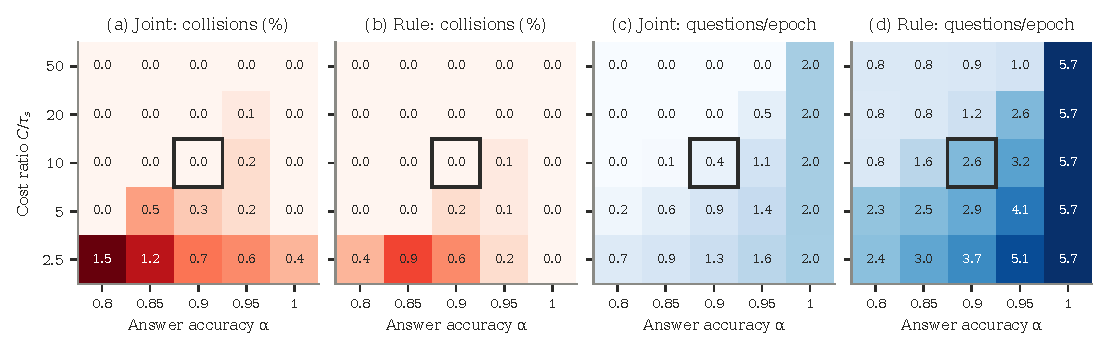
\includegraphics[width=\textwidth]{figures/sensitivity.pdf}
\caption{Sensitivity to the operator's answer accuracy $\alpha$ and the cost ratio $C/\tau_s$ ($N = 6$, noisy tracking, decision-aware calibration, symmetric ask cost, answers drawn per question, 300 epochs per cell; post hoc). (a, b) Collisions per crossing robot (985 crossing robots per cell, so 0.1\% is one collision) for the joint solver and the per-robot rule, both at $\kappa = 1.5$. (c, d) Questions per epoch. The box marks the setting of H4 ($\alpha = 0.9$, $C/\tau_s = 10$).}
\label{fig:sensitivity}
\end{figure*}

\paragraph{Where the delay saving comes from.} The joint solver and the per-robot rule of H1 and H2 differ in two ways. The joint solver decides for the whole epoch, and in its execution mode every robot keeps observing until its decision deadline. The per-robot rule, like the single-robot Ask or Act policy, commits as soon as its probability leaves the asking band, so a robot whose probability rises early stops early, farther from the crossing. The all-stop policy above already suggests that the second difference matters. To separate the two, we ran the joint execution mode without the queue term ($q = 0$) on the same 1{,}000 final epochs. The problem then separates, and each robot applies the per-robot cost rule, but at its deadline; sweeping $\kappa$ traces the grey curves in Fig.~\ref{fig:pareto}. Interpolated to the joint solver's question rate, this deadline rule had a mean delay of 3.87 and \SI{3.99}{s} ($N = 6$ and 8), against 3.80 and \SI{3.93}{s} for the joint solver: coordinating the questions saved 0.068 and \SI{0.052}{s} per robot (paired bootstrap 95\% intervals [0.045, 0.090] and [0.034, 0.070]), whereas deciding at the deadline instead of early saved 2.89 and \SI{3.02}{s}. Neither variant collided. In this setting, therefore, the large H1 and H2 effects measure the value of deferring the decision to the deadline, and the value of joint optimization proper is small, about 2\% of the delay.


\paragraph{Gazebo near-collision validation.} The Gazebo epochs of Section~\ref{sec:res-gazebo} contained no collision, so they could not show that the offline simulator also predicts collisions. We therefore ran a stress set on the same Gazebo set-up: 15 epochs of four robots, all meeting crossing pedestrians (final pool, new seeds), tracking noise 1.5 times the noisy level, operator answers correct with probability 0.9, and three policies chosen to produce close encounters. The always-go policy never stops or asks; the risky policy goes whenever $p_i < 0.5$ and never asks; the third is the joint solver of H1, whose cost model assumes correct answers. Each Gazebo run was replayed offline with the same scenarios, timing and noise seeds (Table~\ref{tab:stress}). All 180 robot runs were valid. Collision outcomes agreed in 98\% of always-go runs, 97\% of joint runs and 90\% of risky runs (Cohen's $\kappa$ 0.65 for the joint solver and 0.69 for the risky policy). The disagreements were concentrated at the threshold: every risky and always-go disagreement had an offline minimum distance within \SI{0.025}{m} of the \SI{0.4}{m} collision distance, and agreement was 61\% for the 18 runs within \SI{0.05}{m} of it, against 99\% for the others. The two joint-solver disagreements were collisions in Gazebo only, both for robots that had asked about a late-turning pedestrian; in Gazebo the robot moved on about \SI{1.2}{s} earlier than offline and passed at 0.37 and \SI{0.39}{m} instead of \SI{0.56}{m}. Minimum distances correlated at 0.93 overall, with a median absolute difference of 0.02--\SI{0.03}{m} for the joint and risky policies. For the always-go policy the difference was larger (median \SI{0.20}{m}) because simulated bodies cannot pass through each other in Gazebo, where 26 of its 60 runs ended in a time-out after contact; the same effect makes delays after a collision incomparable. Among runs without a collision, the mean delay differed by 0.15 and \SI{0.13}{s} for the joint and risky policies. The offline simulator therefore predicts collisions as well as it predicts decisions, apart from encounters that pass within a few centimetres of the threshold.

\begin{table}
\centering
\caption{Gazebo near-collision validation (post hoc): 15 epochs, $N = 4$, crossing pedestrians only, noise $\times 1.5$, $\alpha = 0.9$; 60 robot runs per policy. Agreement and Cohen's $\kappa$ refer to the collision outcome; Risky: goes whenever $p_i < 0.5$. $|\Delta d|$: median absolute difference of the minimum robot--pedestrian distance (m); Near: disagreements whose offline minimum distance was within \SI{0.05}{m} of the collision distance.}
\label{tab:stress}
\begin{tabular*}{\columnwidth}{@{\extracolsep{\fill}}lrrrrrr}
\toprule
 & \multicolumn{2}{c}{Collisions} & & & & \\
\cmidrule(lr){2-3}
Policy & Gz & Off. & Agree & $\kappa$ & Near & $|\Delta d|$ \\
\midrule
Always go & 59 & 60 & 0.98 & -- & 1/1 & 0.20 \\
Risky & 10 & 14 & 0.90 & 0.69 & 6/6 & 0.027 \\
Joint solver & 4 & 2 & 0.97 & 0.65 & 0/2 & 0.020 \\
\bottomrule
\end{tabular*}
\end{table}

\paragraph{Stronger baselines for QAOA.} Table~\ref{tab:qaoabase} compares the probability that each method returns the optimum on the 60 final benchmark instances. Restricting uniform sampling to feasible states or to the $2^N$ halt states already gives most of QAOA's lift: at depth 3, QAOA put 0.062, 0.015 and 0.0033 on the optimum at $N = 4$, 6 and 8, close to the 0.0625, 0.0156 and 0.0039 of uniform sampling over halt states. Conditional on a halt state, the optimum received 0.99, 0.98 and 0.96 times its uniform share (Fig.~\ref{fig:qaoahalt}). Classical methods do much better. A greedy allocation solves the queue formulation exactly: with the queue term, each robot's choice reduces to asking or taking its cheaper non-asking action, the gain from asking falls by $q$ with each additional question, so sorting the robots by their gain from asking and adding questions while the marginal gain stays positive gives the optimum, in $O(N\log N)$ time; it matched the exhaustive solver on all 60 instances and on 2{,}000 random ones. Simulated annealing with one restart of 1{,}000 sweeps found the optimum in 11\%, 3\% and 0.7\% of runs, and with 32 restarts it solved all instances at $N = 4$ but only 65\% at $N = 6$ and 15\% at $N = 8$, probably because the near-degenerate halt states are separated from each other by the exclusion penalty.

\begin{table}
\centering
\caption{Probability of returning the optimum on the 60 final QAOA instances (median over 20 per size; simulated annealing: mean). Halt: every robot asks or stops. Conditional: QAOA probability on the optimum divided by its probability on the halt states.}
\label{tab:qaoabase}
\begin{tabular*}{\columnwidth}{@{\extracolsep{\fill}}lrrr}
\toprule
Method & $N = 4$ & $N = 6$ & $N = 8$ \\
\midrule
Uniform, all states & 0.0039 & 0.00024 & 0.000015 \\
Uniform, feasible states & 0.012 & 0.0014 & 0.00015 \\
Uniform, halt states & 0.063 & 0.016 & 0.0039 \\
QAOA, $p = 1$ & 0.035 & 0.0054 & 0.00080 \\
QAOA, $p = 2$ & 0.058 & 0.013 & 0.0029 \\
QAOA, $p = 3$ & 0.062 & 0.015 & 0.0033 \\
QAOA, $p = 3$, conditional & 0.062 & 0.015 & 0.0038 \\
SA, 1 restart & 0.11 & 0.033 & 0.007 \\
SA, 32 restarts & 1.00 & 0.65 & 0.15 \\
Greedy allocation & 1 & 1 & 1 \\
Exhaustive search & 1 & 1 & 1 \\
\bottomrule
\end{tabular*}
\end{table}

\begin{figure*}
\centering
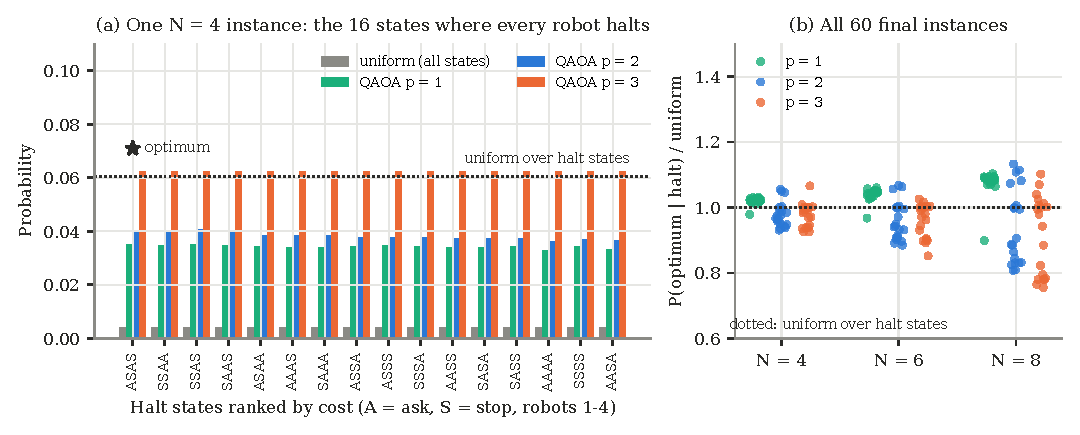
\includegraphics[width=\textwidth]{figures/qaoa_halt.pdf}
\caption{QAOA inside the halt subspace (noiseless, post hoc). (a) One $N = 4$ instance: probability of each of the 16 states in which every robot asks (A) or stops (S), ranked by cost, under uniform sampling over all states and QAOA at depths 1--3; the dotted line marks uniform sampling over the halt states and the star the optimum. (b) Probability on the optimum conditional on a halt state, divided by its uniform value, for the 60 final instances.}
\label{fig:qaoahalt}
\end{figure*}

\subsection{Deviations}
\label{sec:res-dev}

Three deviations from the frozen plan occurred. The $N = 8$ question-rate mismatch in H5 is described above. The exploratory closed-loop stage was run on a 28-core workstation under Python~3.12 and NumPy~2.1.3 rather than the frozen Python~3.13 and NumPy~2.5.3 (scikit-learn as frozen); spot checks in the frozen environment reproduced it exactly, and its rows for the four confirmatory methods equal the confirmatory run robot for robot. The hardware environment used the frozen Qiskit versions under Python~3.12.


\section{Discussion}
\label{sec:discussion}

\paragraph{What coordination buys.} At a fixed number of questions, the joint solver was much faster than per-robot rules that ask equally often (H1 and H2), but the post-hoc decomposition changes what that result means. Almost all of the saving, about \SI{3}{s} per robot, came from observing every pedestrian until the decision deadline instead of committing early, and a per-robot rule applied at the deadline came within 0.05--\SI{0.07}{s} of the joint solver at the same question rate. Pricing the operator's queue does allocate questions better, but with one operator, a service time of \SI{1.5}{s} and at most eight robots per epoch, the queue stays short enough that independent thresholds at the deadline are almost as good. Against the original Ask or Act band the joint solver is slower: that band asks about every uncertain pedestrian and, at six or eight robots, leaves a large share of questions unanswered. The practical lessons are therefore, first, that a fleet sharing an operator should defer its go, yield and ask decisions to a common deadline, and second, that the joint formulation is the natural way to then trade operator load against delay. We expect joint optimization proper to matter more when the operator is scarcer, with longer service times or more robots per epoch, which this study did not test.

\paragraph{Why H4 and H5 failed.} With imperfect answers, the matched comparison does not compare like with like. The $\alpha$-aware joint solver asks about pedestrians with crossing probabilities between about 0.03 and 0.35, and accepts a collision risk of $p_i(1-\alpha)$ for each question, because the cost model values a collision at only ten unnecessary stops. The matched per-robot rule, at $\kappa^\star \approx 6$, asks only between 0.084 and 0.123, almost always about pedestrians who are not crossing, where a wrong answer causes an unnecessary stop rather than a collision. Matching how often the two methods ask did not match whom they ask. The result is therefore partly a statement about the cost ratio $C/\tau_s$: a fleet that must not trade safety for time at this rate needs a larger $C$, a hard constraint on collision risk, or answers verified before acting.

A second, post-hoc observation affects how precise the $\alpha = 0.9$ numbers are. The operator's answers were drawn from a random stream keyed on the scenario, as in the single-robot study and the Gazebo coordinator, so a scenario whose first answer was wrong gave the same wrong answer in every epoch that reused it. All 92 collisions of the $\alpha$-aware joint solver in the confirmatory runs came from eight such crossing scenarios, each reused 12--27 times. With answers drawn per question the same solver collided with 12 crossing robots at each fleet size, from ten scenarios each, and with the symmetric ask cost it met the non-inferiority margin at both sizes (Table~\ref{tab:posthoc}). The confirmatory failure of H4 and H5 is therefore partly an artefact of the answer stream, and the epoch-cluster bootstrap understated the uncertainty of every $\alpha = 0.9$ estimate. It is not only an artefact: the matched rule did not collide under either design, because it asks about pedestrians who are unlikely to be crossing.

\paragraph{Calibration behind an optimizer.} Calibration still matters when decisions are made jointly. With perfect answers, raw probabilities were the only source of collisions, because an overconfident ``not crossing'' score leads the solver to let a robot go without asking. Decision-aware calibration had the fewest collisions in every cell with imperfect answers, but its advantage over conventional calibration was small and not statistically clear here, unlike in the single-robot study \citep{udekwe2026askoract}. One reason is that both calibrations already keep almost every crossing pedestrian above the go threshold of the cost model.

\paragraph{QAOA.} QAOA met its pre-specified criterion, but the post-hoc analysis changes how that result should be read. The lift over uniform sampling is a weak benchmark when most of the search space is obviously bad: the circuits learn the coarse structure of the problem (halt rather than go; never ask and stop at once), which a one-line classical rule also captures, and then spread their probability almost evenly over the remaining $2^N$ states. The part of the problem that coordination is about, which robots should ask given the queue, lives in energy differences of well under 1\% of the spectrum's spread and is not resolved at depths 1 to 3. Future QAOA benchmarks on such problems should report probability within the plausible subspace, or the approximation ratio relative to a strong heuristic, rather than lift over uniform sampling alone; restricting the search to the halt subspace (one qubit per robot) or using constraint-preserving mixers would also put the circuit's resolution where it matters. On hardware the picture is the familiar one \citep{harrigan2021qaoa}: a single layer survives the noise at 8 and 12 qubits, while a second layer at 12 qubits needs 149 two-qubit gates after routing and loses most of its benefit. Nothing here suggests an advantage over classical solvers: the queue formulation is solved exactly by a greedy allocation in $O(N\log N)$ time, and depth-3 QAOA put no more probability on the optimum than uniform sampling over the halt states (Table~\ref{tab:qaoabase}) \citep{abbas2024challenges}. The value of the benchmark is that it uses coefficients from a calibrated perception model, provides an exact reference for every instance, and was specified before the results were known.

\paragraph{Limitations.} Robots run in separate lanes, so the operator is the only coupling; a pairwise corridor-congestion term that we also formulated changed little in development, because robots never shared a lane. Pedestrians are scripted, with eight behaviour families from the single-robot study. The operator model is simple: fixed service time, first come first served, and a fixed answer accuracy. All results are in simulation, with Gazebo agreement as the only physics check. Fleet sizes are small, and the closed-loop policy is solved exactly; QAOA is benchmarked offline, not used in the loop. Each scenario is reused across epochs with the same tracker noise, so every safety statement rests on 400 distinct crossing scenarios per condition, and zero collisions bound the scenario-level rate only below 0.75\%. The pre-registered imperfect-answer runs also reused the operator's answers per scenario. Finally, the cost parameters are a modelling choice, and H4 and Fig.~\ref{fig:sensitivity} show that they matter.


\section{Conclusion}
\label{sec:conclusion}

We formulated the go, yield and ask decisions of a delivery-robot fleet that shares one remote operator as a QUBO with a pairwise queue term, built its coefficients from calibrated pedestrian-intent probabilities, and evaluated it under an analysis plan frozen before the final runs. With perfect operator answers, the joint solver cut mean delay per robot by about \SI{3}{s} against per-robot rules that ask equally often, without collisions in more than 3{,}000 encounters with crossing pedestrians; a post-hoc decomposition attributes almost all of this saving to deciding at a common deadline rather than early, with joint optimization of the questions adding 0.05--\SI{0.07}{s}. With imperfect answers the pre-specified non-inferiority hypotheses failed. Post hoc, part of that failure traced to operator answers that were reused across epochs; with answers drawn per question and both kinds of operator error priced, the joint solver met the margin, although the matched rule still had no collisions, and a per-robot risk cap removed the collisions at the price of not asking at all. Calibration remained necessary behind the optimizer. QAOA met its pre-specified benchmark in noiseless simulation and kept a clear gain over random sampling on IBM hardware at depth 1, but its gain comes from concentrating on states in which every robot halts, not from choosing which robots should ask, and a greedy classical allocation solves the problem exactly. Useful next steps are settings in which the operator is the binding constraint, a shared-lane simulator in which robots also interact physically, measured human response times and error rates, and a larger pool of distinct scenarios, so that safety can be bounded at the scenario level.

\section*{Data availability}
The code, the frozen analysis plan (tag \texttt{v2-prereg}), development results, all final results and the post-hoc analyses (\texttt{results/posthoc}) are available at \url{https://github.com/daniel-udekwe/ask-act-v2}.

\section*{Declaration of competing interest}
The authors declare that they have no known competing financial interests or personal relationships that could have appeared to influence the work reported in this paper.

\section*{CRediT authorship contribution statement}
\noindent\textbf{Daniel Udekwe:}  conceptualization, methodology, software, formal analysis, writing -- original draft. \textbf{Qianwen (Vivian) Guo:} supervision, writing -- review and editing.

\bibliographystyle{cas-model2-names}

% Loading bibliography database
\bibliography{cas-refs}

\end{document}
